                        %%%%%   PREAMBLE  %%%%%
%%%%%%%%%%%%%%%%%%%%%%%%%%%%%%%%%%%%%%%%%%%%%%%%%%%%%%%%%%%%%
%% HEADER
%%%%%%%%%%%%%%%%%%%%%%%%%%%%%%%%%%%%%%%%%%%%%%%%%%%%%%%%%%%%%

% \documentclass[12p,spanish,a4paper,oneside]{article}%Paquete de idioma español, problema con la separación de palabras
% Alternative Options:
%	Paper Size: a4paper / a5paper / b5paper / letterpaper / legalpaper / executivepaper
% Duplex: oneside / twoside
% Base Font Size: 10pt / 11pt / 12pt
\documentclass{beamer}
\usetheme{Darmstadt}
\usecolortheme{sidebartab}
\usepackage[sort]{natbib}

\usepackage{authblk}

%% Language %%%%%%%%%%%%%%%%%%%%%%%%%%%%%%%%%%%%%%%%%%%%%%%%%
\usepackage[spanish,activeacute]{babel} % english francais, polish, spanish, ...
\usepackage[T1]{fontenc}
%\usepackage[utf8]{inputenc} % Para uso en ingles
\usepackage[utf8]{inputenc}	%Para poder ingresar acentos y demás directamente
\usepackage{verbatim}%Paquete para poder comentar oraciones completas
% Por problemacon el idioma en las referencias ??
%\renewcommand\refname{{\large Referencias}} 
%\newcommand\VRule[1][\arrayrulewidth]{\vrule width #1}

\usepackage{lmodern} %Type1-font for non-english texts and characters

%% Packages for Graphics & Figures %%%%%%%%%%%%%%%%%%%%%%%%%%
\usepackage{graphicx} %%For loading graphic files
\usepackage{wrapfig} %% For text next to graphics
\usepackage{subfigure} %% Subfiguras
\usepackage[small,bf]{caption} %% Cambio de formato de los captions
%\usepackage{subfig} %%Subfigures inside a figure
%\usepackage{tikz} %%Generate vector graphics from within LaTeX
\usepackage{epsfig}

%% Please note:
%% Images can be included using \includegraphics{filename}
%% resp. using the dialog in the Insert menu.
%% 
%% The mode "LaTeX => PDF" allows the following formats:
%%   .jpg  .png  .pdf  .mps
%% 
%% The modes "LaTeX => DVI", "LaTeX => PS" und "LaTeX => PS => PDF"
%% allow the following formats:
%%   .eps  .ps  .bmp  .pict  .pntg


%% Line Spacing %%%%%%%%%%%%%%%%%%%%%%%%%%%%%%%%%%%%%%%%%%%%%
%\usepackage{setspace}
%\singlespacing        %% 1-spacing (default)
%\onehalfspacing       %% 1,5-spacing
%\doublespacing        %% 2-spacing


%% Other Packages %%%%%%%%%%%%%%%%%%%%%%%%%%%%%%%%%%%%%%%%%%%
%\usepackage{a4wide} %%Smaller margins = more text per page.
%\usepackage{fancyhdr} %%Fancy headings
%\usepackage{longtable} %%For tables, that exceed one page
%\usepackage{authblk} % For multi author affiliation support.
\newcommand\Mark[1]{\textsuperscript#1}

%% Math Packages %%%%%%%%%%%%%%%%%%%%%%%%%%%%%%%%%%%%%%%%%%%%
\usepackage{amsfonts}
\usepackage{amssymb,amsmath}
\usepackage{wasysym}
\usepackage{arcs} % Para poder escribir arcos... increible.
%\usepackage[amsthm,hyperref,thref]{ntheorem}


\usepackage{fancyhdr}
\renewcommand{\headrulewidth}{1pt}  %  línea horiz. bajo el encabezado
\renewcommand{\footrulewidth}{1pt}  %  línea horiz. sobre el pie



% \usepackage{makeidx}

%\usepackage{times}
%\usepackage[OT1,T1]{fontenc}

\usepackage{palatino}
% palatino: una fuente excelente, pero si sale
% mal en el .pdf descomentar las dos líneas anterires


%% Reseteo de Margenes
%\usepackage{vmargin}
%\setpapersize{A4}
%\setmarginsrb{2.5cm}{2cm}{1.5cm}{2cm}%
%{1cm}{1cm}%
%{1cm}{1cm}

%% Mejora de visualización
\usepackage{color}       % Para el color de las fuentes
\usepackage{lettrine}    % Letra capital
\usepackage{enumerate}   % Entorno enumerate mejorado
\usepackage{mdwlist}     % Entorno descripcion mejorado
\usepackage{hyperref}
\usepackage{datetime}	
\usepackage{listings}	 % Mejora de entorno para mostrar códigos
%\usepackage{paralist}	  
%\usepackage[framed,numbered,autolinebreaks,useliterate]{mcode}
%\usepackage[autolinebreaks,useliterate]{mcode}% Paquete de matlab para poder agregar el codigo
  

%\parskip 0.15cm          %  Queda mejor pero mas paginas


%\usepackage{appendix}	% Usando paquete de apendices

\usepackage{array,booktabs}
\usepackage{multirow}

% Para permitir un nuevo nivel de sectionado
\setcounter{secnumdepth}{5}

\usepackage{float}
\usepackage[toc]{appendix}


% CUSTOM COMMANDS 
% TODO NOTES
\usepackage{todonotes} % PARA AGREGAR NOTAS 'TODO' DENTRO DEL PDF
\newcommand{\todosection}[0]{\todo[inline]{Desarrollar Sección \thesection}}
\newcommand{\todosubsection}[0]{\todo[inline]{Desarrollar Subsección \thesubsection}}
\newcommand{\pendiente}[1]{\todo[inline]{\textbf{Pendiente:} #1}}
\newcommand{\pendpres}[1]{\todo[inline, size=\tiny]{{\textbf{Pendiente:} #1}}}

% CUSTOM COMMANDS
\newcounter{designlayer}
\newcommand{\designlayer}[2]{
	\refstepcounter{designlayer}\label{#2}
	\subsection{Etapa \thedesignlayer: #1}
}

\newcounter{requirement}
\newcommand{\requirement}[1]{
	\refstepcounter{requirement}\smallskip
	\textbf{Requerimiento \therequirement: }{{#1}.\smallskip}
}

\newcounter{activity}
\newcommand{\activity}[2]{
	\refstepcounter{activity}\smallskip \label{ac:#1}
	\textbf{Actividad \theactivity~(#1): }{#2.\smallskip}
}
\newcommand{\acref}[1]{
	{\textbf{A\ref{ac:#1} (#1)}}
}

\newcounter{component}
\newcommand{\component}[2]{
	\refstepcounter{component}\smallskip \label{cp:#1}
	\textbf{Componente \thecomponent~(#1): }{{#2}.\smallskip}
}
\newcommand{\cpref}[1]{
	{\textbf{C\ref{cp:#1} (#1)}}
}
%\title[Diseño de Plataforma Móvil]{Proceso de Diseño de una Plataforma Móvil para el transporte de Materiales}
%\author[1,2]{ {{\large{Guillermo Rolle}} \thanks{grolle@fceia.unr.edu.ar}} }
\author[1,2]{Guillermo Rolle}
%\author[2]{ {\large{Alberto Rolle}} }
\affil[1]{LAC, FCEIA, UNR \authorcr \small{\emph{Riobamba 250bis, Rosario, Argentina}}}
\affil[2]{CONICET}
\title[Diseño de Plataforma Móvil]{Proceso de Diseño de una Plataforma Móvil para el transporte de Materiales}


\AtBeginSection[]{
	\begin{frame}
		\vfill
		\centering
		\begin{beamercolorbox}[sep=8pt,center,shadow=true,rounded=true]{title}
			\usebeamerfont{title}\insertsectionhead\par%
		\end{beamercolorbox}
		\vfill
	\end{frame}
}

\AtBeginSubsection[]{
	\begin{frame}
		\vfill
		\centering
		\begin{beamercolorbox}[sep=8pt,center,shadow=true,rounded=true]{subtitle}
			\usebeamerfont{subtitle}\insertsubsectionhead\par%
		\end{beamercolorbox}
		\vfill
	\end{frame}
}

\AtBeginSubsubsection[]{
	\begin{frame}
		\vfill
		\centering
		\begin{beamercolorbox}[sep=8pt,center,shadow=true,rounded=true]{title}
			\usebeamerfont{title}\insertsubsectionhead\par%
		\end{beamercolorbox}
		\begin{beamercolorbox}[sep=8pt,center,shadow=true,rounded=true]{subtitle}
			\usebeamerfont{subtitle}\insertsubsubsectionhead\par%
		\end{beamercolorbox}
		\vfill
	\end{frame}
}

\usepackage{multicol}


\begin{document}	
	\frame[plain]{\titlepage}
	
	\section*{Contenidos}
	\frame[t]{\frametitle{Contenidos de la Presentación} \small \smaller 
		    \begin{columns}[t]
			\begin{column}{.5\textwidth}
				\tableofcontents[sections={1-2}]
			\end{column}
			\begin{column}{.5\textwidth}
				\tableofcontents[sections={3-5}]
			\end{column}
		\end{columns}
		}
	
	\section{Desarrollo}
%	\frame[t]{\frametitle{Desarrollo Específico}
%	\tableofcontents[currentsection,sectionstyle=hide]
%	}
	
	\designlayer{Análisis de las necesidades del cliente}{dl:cliente}
	\subsubsection{Misión Global}
	\frame[t]{\frametitle{\insertsubsubsectionhead}
	\begin{quote}
		El sistema debe permitir el traslado de materiales, productos y subproductos autónomamente entre el almacén y estaciones de producción internas a la fábrica, garantizando la seguridad de operarios y/o otros humanos,	integridad de los materiales transportados y eficiencia.
		
		La solución requerida es un prototipo que priorice los bajos costos de fabricación y la simplicidad del diseño y funcionamiento. Además, se prevé modularidad para que en primera instancia pueda ser utilizado de forma manual pero permita el agregado de módulos que mejoren las funcionalidades y automatización a posterior sin necesidad de rediseñar todo el sistema.
		\end{quote}
	}
	
	\subsubsection{Requerimientos del Cliente}
	\frame[t]{ \frametitle{\insertsubsubsectionhead} {\smaller \par
	\begin{enumerate}
	\item {El sistema debe transportar materiales (entre otras): bolsas con resortes de 30kg c/u de tamaño 50cm x 50cm x 15cm; bolsas grimar de 22kg c/u; bolsas de estantería de 20kg c/u}
	\item{La carga admisible máxima a transportar es de 100kg}
	\item{El sistema debe circular por la fábrica}
	\item{La solución debe requerir la mínima modificación de las instalaciones existentes de la fábrica}
	\item{El sistema debe ser ergonómico para los operarios}
	\item{El sistema debe ser capaz de maniobrar seguramente}
	\item{El sistema debe garantizar la integridad de los materiales transportados}
	\item{El sistema debe reconfigurable en cuanto al sistema de locomoción y estructuras de operación}
	\item{El sistema debe tener el mínimo costo}
	\item{El sistema debe ser eficiente}
	\item{El sistema debe permitir su uso manual y debe permitir agregarle funcionalidades modularmente con distintos niveles de autonomía}
	\end{enumerate}
}\par
	}
	
	\subsubsection{Requerimientos del Entorno}
	\frame[t]{ \frametitle{\insertsubsubsectionhead}
		\framesubtitle{Contexto del Sistema}
	\begin{figure}[H]
		\centering
		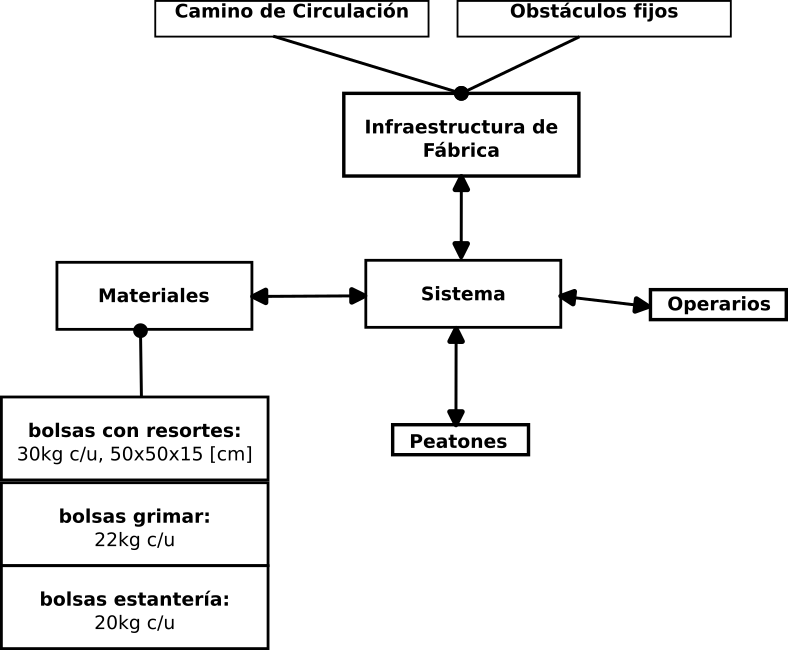
\includegraphics[width=0.6\textwidth]{figs/context}
		\caption[Diagrama de Contexto]{Diagrama de Contexto e Interacción del Sistema}
		\label{fig:contextodelsistema}
	\end{figure}
	
%	\pendpres{{Mejorar Imagen}}
	}
	
	\frame[t]{ \frametitle{\insertsubsubsectionhead} \smaller
		\textbf{Requerimientos del Entorno}
		\begin{enumerate}
			\item{La velocidad máxima admisible para transitar de forma segura es de 2m/s ($\approx$ 7.2km/h), según Norma \textit{NN}}
			\item{El sistema debe superar satisfactoriamente irregularidades del suelo (escalones/pozos) de hasta 1.5cm de alto}
			\item{El sistema debe transitar por pendientes del suelo de hasta 15°}
			\item{El sistema debe circular por dentro de los senderos: el ancho de éstos es de 1m y el radio interno de las curvas es de 0.1m}
		\end{enumerate}
	}
	
	\designlayer{Diseño Conceptual}{dl:dc}
	
	\subsubsection{Arquitectura Funcional}
	\frame[t]{
		\frametitle{\insertsubsubsectionhead} 
		\framesubtitle{Análisis conceptual de Funcionalidades}
%		\hrule
%		\begin{center}
		\begin{columns}[T]
%			\begin{column}{0.5\textwidth}
%%					\begin{center}
%%					\hrule
%					\centering
%%					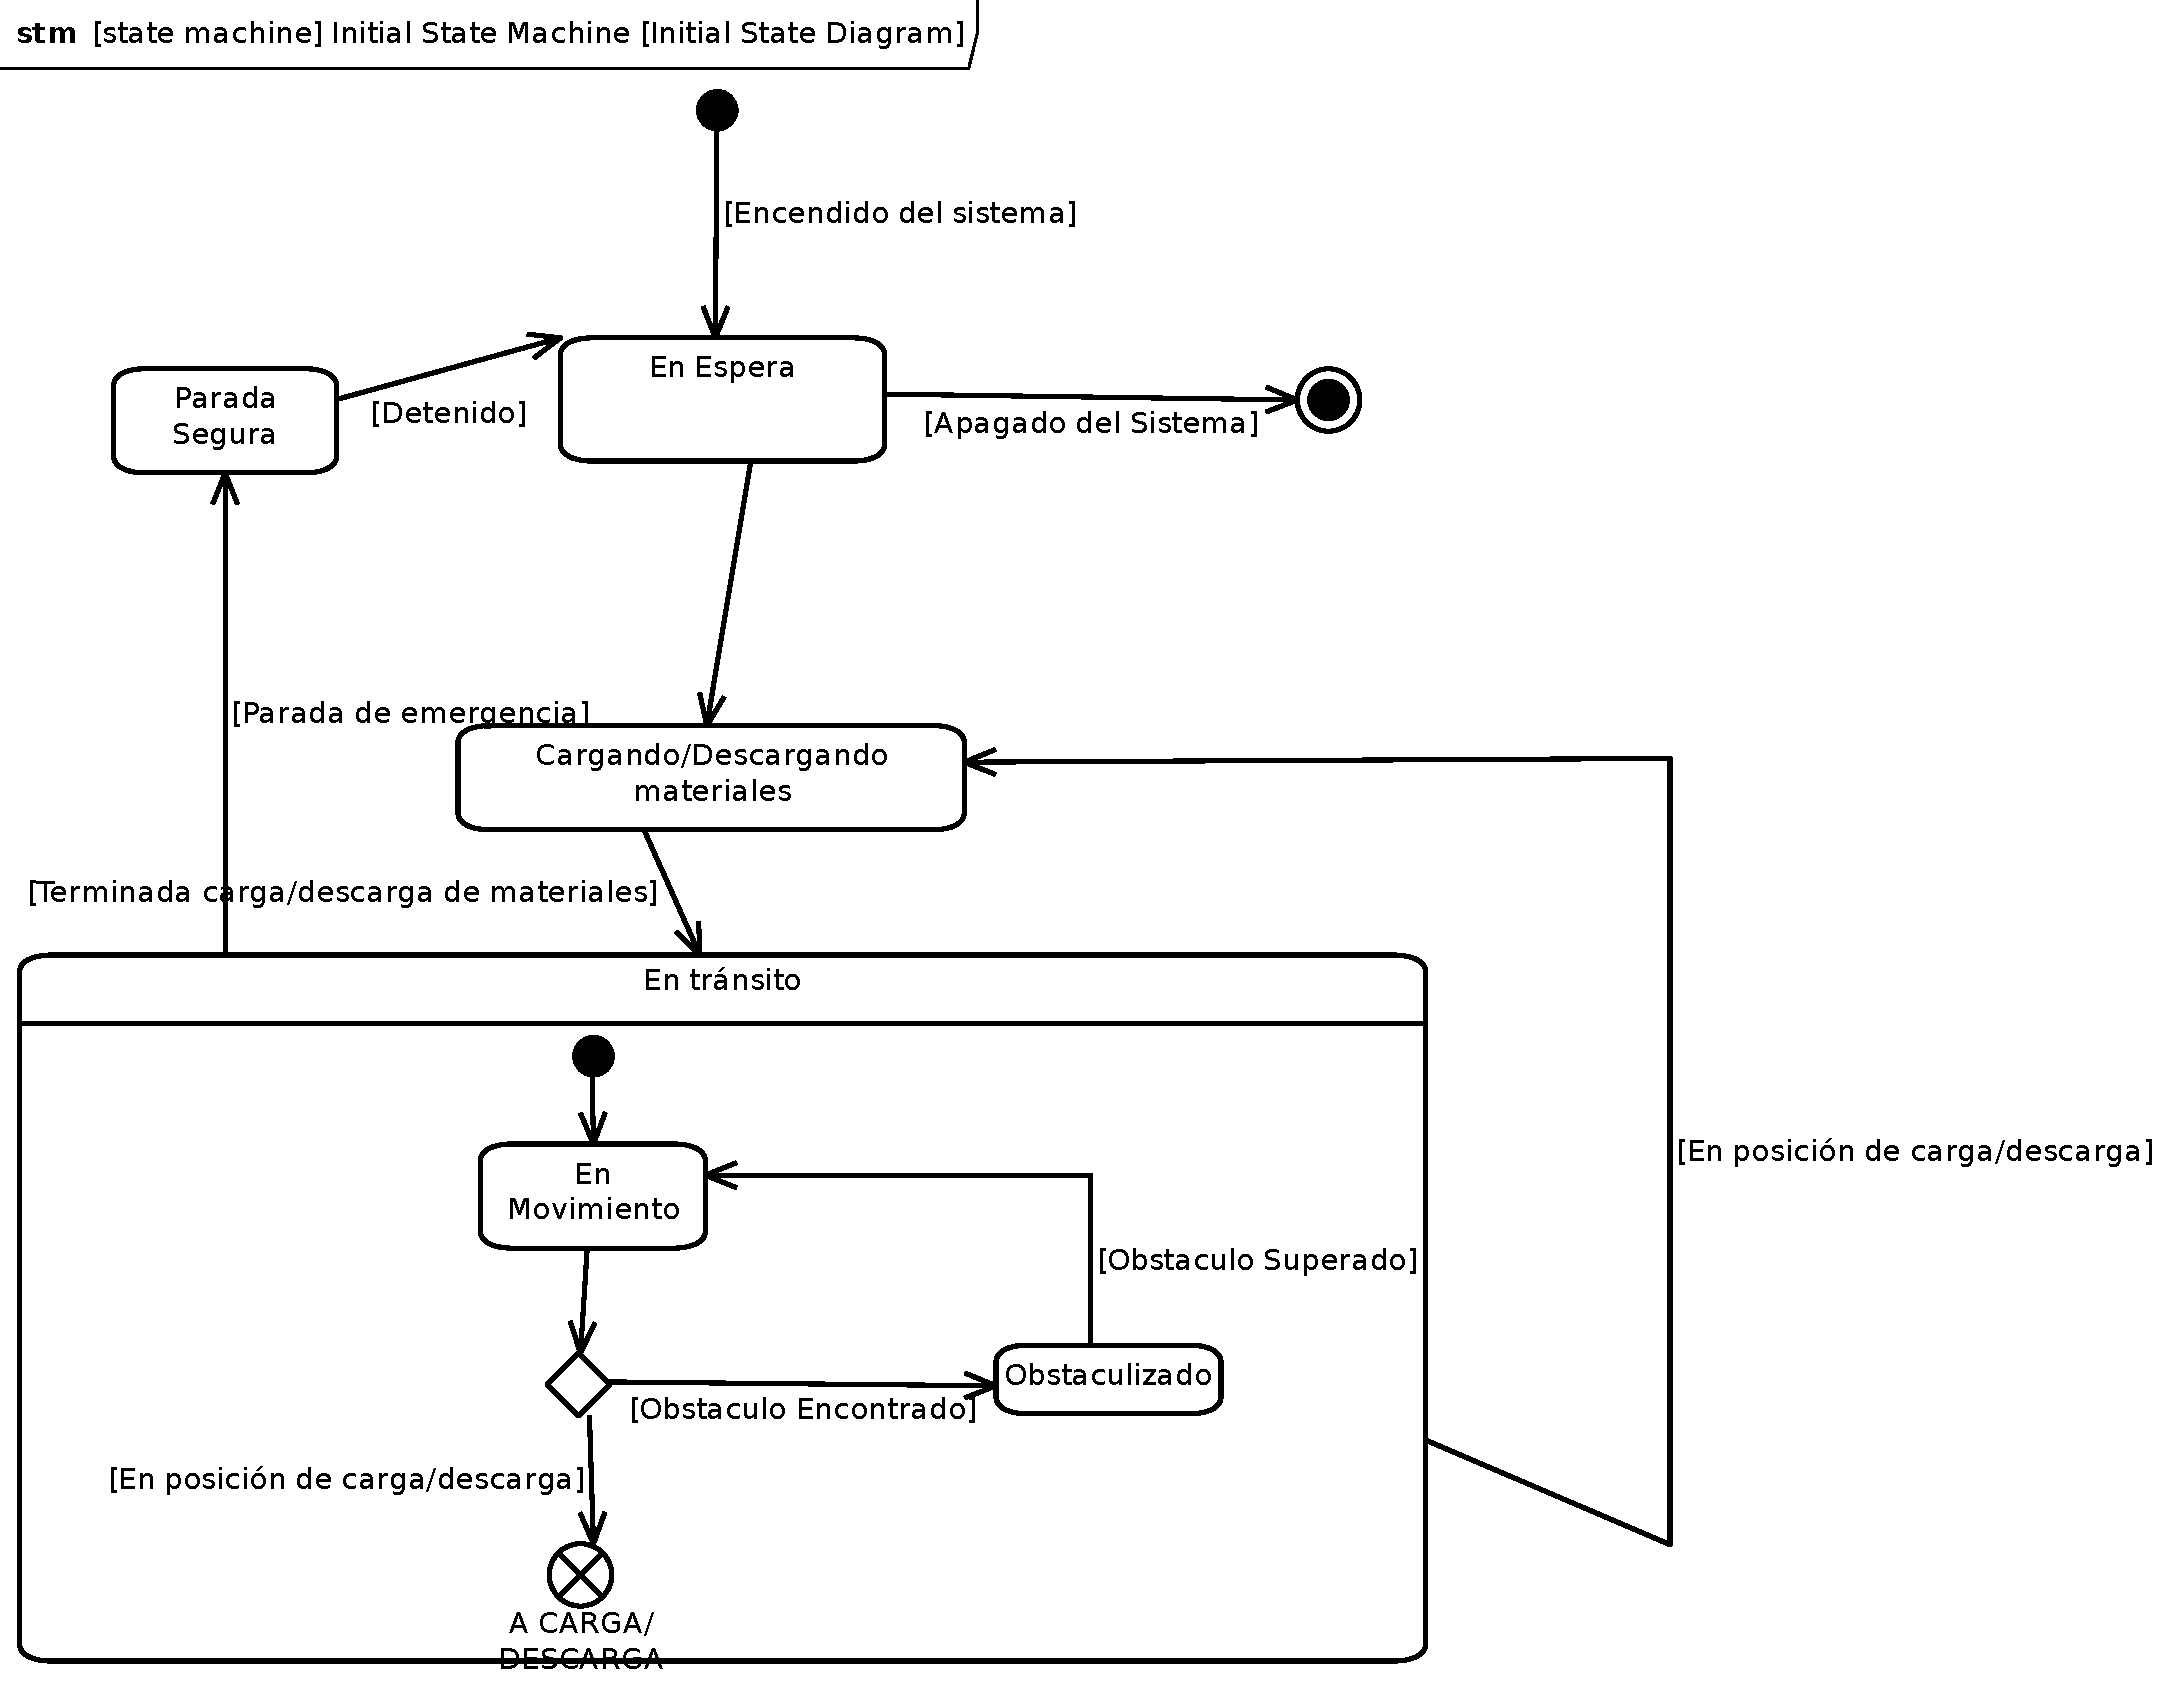
\includegraphics[width=1\textwidth]{figs/Initial_State_Diagram.pdf}
%%					\hrule
%%					\end{center}
%%				
%			\end{column}
			\begin{column}{0.7\textwidth}
				\begin{center}
%					\pendpres{Mejorar Imágenes}
					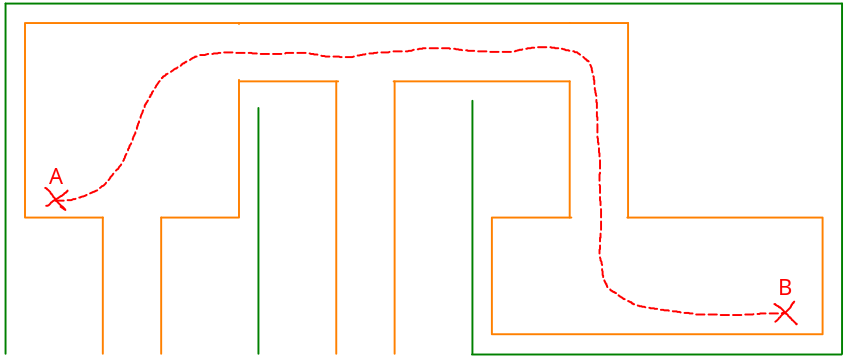
\includegraphics[width=1\textwidth]{figs/f1AB.png}
				\end{center}
			\end{column}
		\end{columns} \bigskip
%		\end{center}
%		\hrule
%		\begin{quote}
			{ \scriptsize
			\par \textit{<<El sistema está quieto. Recibe una orden de para ir desde su ubicación actual A hasta una ubicación B. Debe trasladarse seguramente por los caminos demarcados del suelo de la fábrica.  Si se encuentra con algún 			obstáculo debe evadirlo o detenerse. Cuando llega a B debe detenerse nuevamente. En este momento, se queda quieto/frenado hasta que esté cargado con materiales. Una vez cargado, recibe la orden de ir hacia un nuevo punto y repite el ciclo de trabajo>>}
			\par
		}
%		\end{quote}
	}
	
	\frame[t]{\frametitle{\insertsubsubsectionhead}
		\framesubtitle{Descomposisión en actividades}
		{\tiny \par
		\begin{enumerate}	
			\item \textbf{Marcha: }{Es la posibilidad de andar o trasladarse por el entorno. Implica el movimiento de las ruedas (rotación/dirección)}
			\item \textbf{Mantenerse Estático: }{Es la posibilidad de mantenerse completamente estático ante esfuerzos externos durante el momento de carga o descarga de materiales}
			\item \textbf{Manipulación de Materiales: }{Consiste en la posibilidad en sí cargar, trasladar y descargar los materiales. Puede ser, por ejemplo, soportarlos sobre el chasis, acoplarse a un tráiler que tenga los materiales, empujando/llevando una estantería, pallets, etc. Las subactividades de carga y descarga dependen del tipo de traslado seleccionado}
			\item \textbf{Modularidad Mecánica: }{Distintos módulos acoplables le permitirán efectuar las actividades~1 a~3 de distintas maneras}
			\item \textbf{Gestión de Energía: }{El sistema tener autonomía energética (baterías) y debe convertirla a energía mecánica para efectuar el trabajo correspondiente. Además, las baterías se deben poder recargar}
			\item \textbf{Planeamiento de Trayectorias: }{El sistema debe determinar la trayectoria de referencia entre los puntos A y B}
			\item \textbf{Localización: }{El sistema debe poder localizarse y ubicarse dentro de la fábrica}
			\item \textbf{Recolección de Datos: }{El sistema recopila datos de sensores introceptivos (velocidad de las ruedas, consumo eléctrico, estado de baterías, etc.) y de sensores exteroceptivos (cámaras, sensores de distancias, cámaras térmicas, GPS, antenas de radio, etc.)}
			\item \textbf{Evasión de obstáculos: }{El sistema debe evadir obstáculos y/o detenerse de forma segura, alertando a los operarios}
			\item \textbf{Parada de Emergencia: }{El sistema debe poder ser detenido fácil y rápidamente por un operario en caso de emergencias}
		\end{enumerate}
		\par
		}
	}
	
	\subsubsection{Arquitectura Lógica}
	\frame[t]{\frametitle{\insertsubsubsectionhead}
		\framesubtitle{Alojamiento de Funciones en Componentes o Bloques}
		{\tiny \par
			\begin{enumerate}	
				\item \textbf{Sistema de Locomoción: }{Ejecuta la Actividad~\textbf{Marcha}. Propiedades internas: tipo (ruedas, orugas o patas), cantidad y tipos de apoyos, configuración cinemática}

				\item \textbf{Sistema de Frenado: }{Ejecuta la Actividad~\textbf{Mantenerse Estático}. Propiedades internas: Modo de frenado (freno electrónico de motores, brazos desplegables, apoyar el chasis contra el suelo, frenos pedales en las ruedas o chasis)}
				
				\item \textbf{Sistema de Materiales}{Ejecuta la actividad~\textbf{Manipulación de Materiales}. Propiedades internas: método de traslación, método de carga, método de descarga}
				
				\item \textbf{Sistema de Control: }{Ejecuta las Actividades~\textbf{Localización}, \textbf{Planeamiento de Trayectorias} y~\textbf{Evasión de obstáculos}. Comanda al Componente~\textbf{Sistema de Locomoción} a través del componente~\textbf{Sistema de Energía} y recibe información de~\textbf{Sistema de Sensores}. Propiedades internas: Controladores de alto/bajo nivel, Computadora SBC, etc.}
				
				\item \textbf{Sistema de Sensores: }{Ejecuta las actividades de \textbf{Recolección de Datos} y envía información a~\textbf{Sistema de Control}. Propiedades internas: cantidades y tipos de sensores (sensores de velocidad, sensores de distancia, IMUs, cámaras, etc.). Recibe información del Sistema de Locomoción y otras fuentes}.
				
				\item \textbf{Sistema de Energía: }{Ejecuta las actividades de~\textbf{Gestión de Energía}. Alimenta a todos los demás sistemas que lo requieran y es comandado por el \textbf{Sistema de Control}. Propiedades internas: Baterías, interruptores, PWM, tipo de motores (DCM, STEPPER, etc.), tipo de reductores etc.}
				
				\item \textbf{Sistema de Emergencias: }{Ejecuta las actividades~\textbf{Parada de Emergencia}. Comanda al Sistema~\textbf{Sistema de Energía}. Propiedades internas: botón de emergencias, algoritmo de parada de emergencia segura}
				
				\item \textbf{Interfaz: }{Este componente permite comunicarse a través con el exterior (operarios). Permite enviar y recibir señales. Propiedades internas: luces, alarmas sonoras, pantalla, teclado de entrada.}
				
				\item \textbf{Estructura Mecánica: }{Este componente representa la estructura mecánica en sí. Los otros sistemas tendrán una parte físico-mecánica (ocupan espacio). La estructura mecánica debe ser modular y reconfigurable y alojar los componentes físicos de todos los otros sistemas}
			\end{enumerate}
			\par
		}
	}
	\frame[c]{ \frametitle{\insertsubsubsectionhead}
		\framesubtitle{Modelo de Cebolla}
		\small \smaller
		\begin{columns}[c]
			\begin{column}{0.4\textwidth}
				\begin{figure}[H]
					%			\pendpres{Mejorar Imágenes}
					\centering
					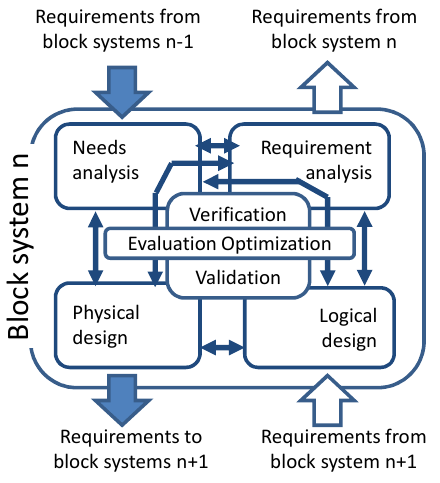
\includegraphics[width=1\textwidth]{figs/blockmodeling.png}
					\caption{\small \smaller Modelado de Bloques recursivo \cite{lo_needs_2012}}
				\end{figure}
			\end{column}
			\begin{column}{0.6\textwidth}
				\begin{figure}[H]
					%			\pendpres{Mejorar Imágenes}
					\centering
					\includegraphics[width=0.9\textwidth]{figs/onion1.png}
					\caption{\small \smaller Modelo de Cebolla}
				\end{figure}
			\end{column}
		\end{columns}
	}
	
	\subsubsection{Estructura Física}
	\frame[t]{ \frametitle{\insertsubsubsectionhead}
		\framesubtitle{Análisis de Alternativas}
		\begin{enumerate}
			\item Para cada componente identificado se listan posibles alternativas solución.
			\item Se definen criterios de evaluación para seleccionar la mejor en cada caso.
			\item Se define un método de evaluación
			\item Se evalúan todas las alternativas
			\item Se elije la mejor			
		\end{enumerate}
		
		\vfill
		\textbf{Nota: } La evaluación de alternativas puede también aparecer durante el análisis funcional o en otras etapas de diseño. Es un proceso que ocurre todo el tiempo.
	}
	
	\frame[t]{ \frametitle{Sistema de Locomoción}
		\framesubtitle{Descripción de Alternativas}
		\small 
		\begin{columns}[t]
			\begin{column}{0.5\textwidth}
				\begin{itemize}
					\item Método de Propulsión:
					\begin{enumerate}
						\item Ruedas
						\item Orugas
						\item Patas
					\end{enumerate}
					\item Modelo Cinemático (para ruedas y orugas) (ver Figura)
				\end{itemize}
			\end{column}
			\begin{column}{0.5\textwidth}
				\begin{itemize}
				\item Cantidad de ruedas/apoyos:
				\begin{enumerate}
					\item 1 apoyo
					\item 2 apoyos 
					\item 3 apoyos
					\item 4 apoyos
				\end{enumerate}
				
			\end{itemize}
		\end{column}
		\end{columns}
		
		\centering 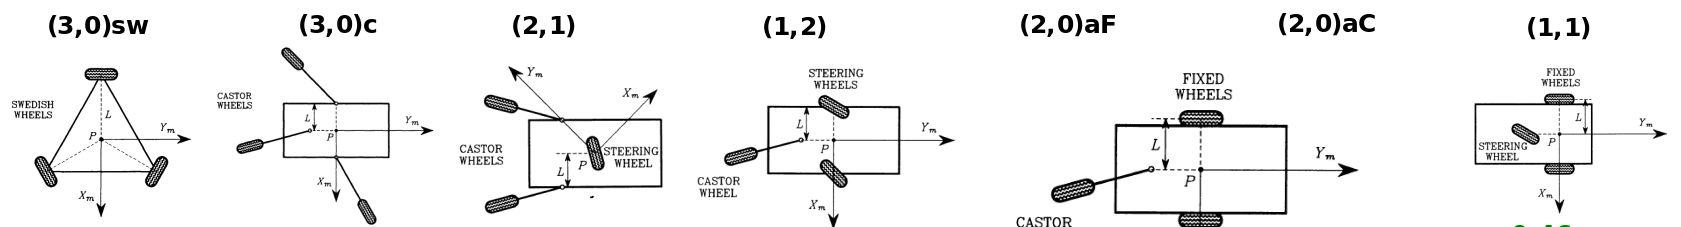
\includegraphics[width=1\textwidth]{figs/confcinematica.png}
		\begin{itemize}
			\item Configuración de Actuadores (para ruedas): Cuáles, cuántas y cómo deben ser actuadas las ruedas motrices
		\end{itemize}
}
	
%	\paragraph{Sistema de Locomoción}
	\frame[t]{ \frametitle{Sistema de Locomoción}
		\framesubtitle{Método de Evaluación}
		
%		{\tiny \par{
		\textbf{Criterios de Evaluación (MOEs): }
		\begin{itemize}
			\item Capacidad de Maniobrar \cite{de_wit_theory_1996}
			\begin{itemize}
				\item Grado de Movilidad 
				\item Grado de Maniobrabilidad 
			\end{itemize}
			\item Simplicidad del diseño
			\begin{itemize}
				\item Tipos de ruedas y cantidades: Las ruedas direccionables requieren un diseño más complejo del alojamiento
				\item Homogeneidad de actuadores: de rotación y/o dirección
				\item Cantidad y complejidad de partes móviles a diseñar
			\end{itemize}
			\item Estabilidad
			\item Costo
			\begin{itemize}
				\item Cantidad de actuadores
				\item Costo de componentes (a comprar)
			\end{itemize}
		\end{itemize}
		\textbf{Método de Toma de Decisiones: } AHP (Analytic Hierarchy Process)
	}
	
	\frame[c]{ \frametitle{Sistema de Locomoción}
		\framesubtitle{Analytic Hierarchy Process}
%		\centering 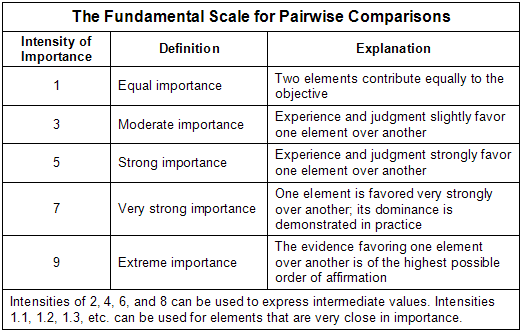
\includegraphics[width=0.39\textwidth]{figs/AHPFundamentalScale.png}
		{\centering 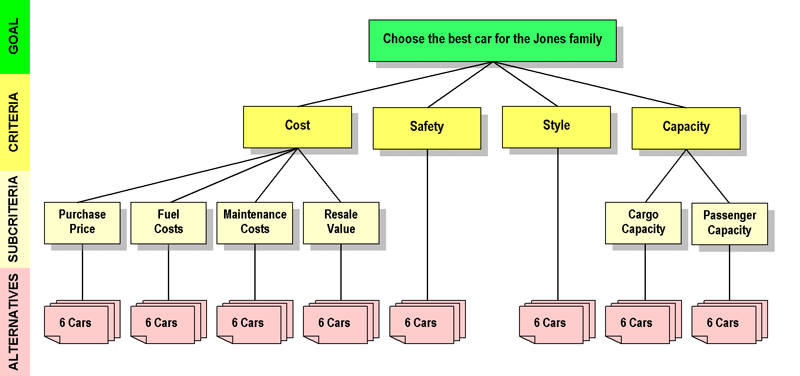
\includegraphics[width=0.9\textwidth]{figs/AHPJones01.png}} \\
		\small \smaller \textbf{Resumen del Método: } Para cada bloque de un mismo nivel (criterios y alternativas) se hacen comparaciones 1vs1, se forman matrices de prioridades y se evalúan puntajes finales ponderados para cada posible alternativa.\\
		\textbf{Escala Fundamental de Comparaciones: } Se asignan valores del 1 (igual importancia entre elementos) al 9 (extrema importancia favorecer un elemento). 
	}
	
%	}\par }
		
		\frame[t] {
			\frametitle{Sistema de Locomoción}
			\framesubtitle{Resultados de Evaluación}
			\centering
			{\tiny
%				\begin{center}
					\begin{tabular}{|c|c|c|c|c|}
						\hline
						& \multicolumn{4}{c|}{iDDP} \\
						\hline
						DA & Propulsión & Apoyos & Familia & Subconf. \\
						\hline
						5 & RUEDAS & 3 & (3,0) & Cáster \\
						\hline
						6 & RUEDAS & 3 & (2,1) & - \\
						\hline
						7 & RUEDAS & 3 & (1,2) & - \\
						\hline
						8 & RUEDAS & 3 & (2,0) & Actuadas fijas \\
						\hline
						9 & RUEDAS & 3 & (2,0) & Actuada cáster \\
						\hline
						10 & RUEDAS & 3 & (1,1) & - \\
						\hline
						12 & RUEDAS & 4 & (2,0) & - \\
						\hline
						14 & ORUGAS & 2 & (2,0) & - \\
						\hline
					\end{tabular}
%				\end{center}
			} \vspace{3mm} 
			\\
			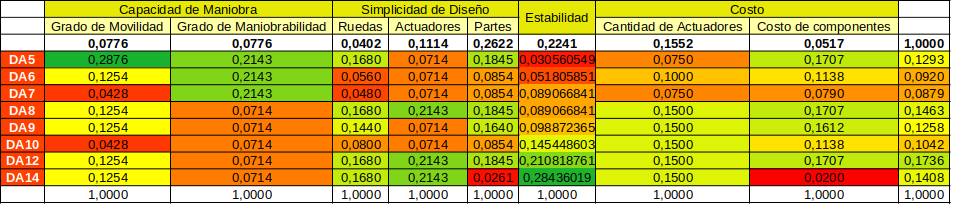
\includegraphics[width=1\textwidth]{figs/evsloc000.png}
		{\smaller
			\textbf{Solución adoptada DA12}: configuración de 4 ruedas con tracción diferencial con actuadores en las ruedas fijas.
		}
	}
	
	\frame[t]{ \frametitle{Sistema de Frenado}
		\framesubtitle{Descripción de Alternativas}
		\begin{itemize}
			\item Freno electrónico por control de motores
			\item Pedal de freno en las ruedas (requiere Sist. Locomoción con Ruedas)
			\item Brazos desplegables
			\item Tornillos de apoyo manuales 
			\item Mecanismo de descenso del chasis / elevación de las ruedas
		\end{itemize}
		\begin{quote}
		Por simplicidad, en primera instancia se utilizará freno por control de los motores con la opción de pedal de freno en una rueda cáster. Se debe prever que la estructura mecánica pueda aceptar módulos de frenado diferentes en el futuro.
		\end{quote}
	}
	
	\frame[t]{ \frametitle{Sistema de Materiales}
		\framesubtitle{Descripción de Alternativas}
		\begin{enumerate}
			\item \textbf{Sobre Chasis:} Materiales transportados directamente sobre el chasis
			\item \textbf{Tipo Trailer:} requiere diseñar un carro móvil con un chasis que soporte la carga. Teniendo en cuenta la modularidad y reconfiguración del sistema, es un caso del primero. Tiene muy baja maniobrabildad.
			\item \textbf{Transporte de estanterías:} Las estanterías no son motorizadas pero son móviles con ruedas. El carro se mete debajo y mediante un mecanismo se fijan entre sí y se desplazan en conjunto. La principal limitación radica en el tamaño total requerido para esta solución.
		\end{enumerate}
	}
	
	\frame[c]{ \frametitle{\insertsubsubsectionhead}
		\framesubtitle{Conjunto de Alternativas Finales}
		
		\begin{columns}[c]
			\begin{column}{0.5\textwidth}
				Una vez que las alternativas para cada componente fueron propuestas, analizadas, y evaluadas según ciertos criterios, se puede expandir el modelo de cebolla, ahora teniendo bloques o componentes descriptos de forma más detallada verificando la integración entre todos los nuevos componentes y verificación de los requisitos.
			\end{column}
			\begin{column}{0.5\textwidth}
				\begin{center}
					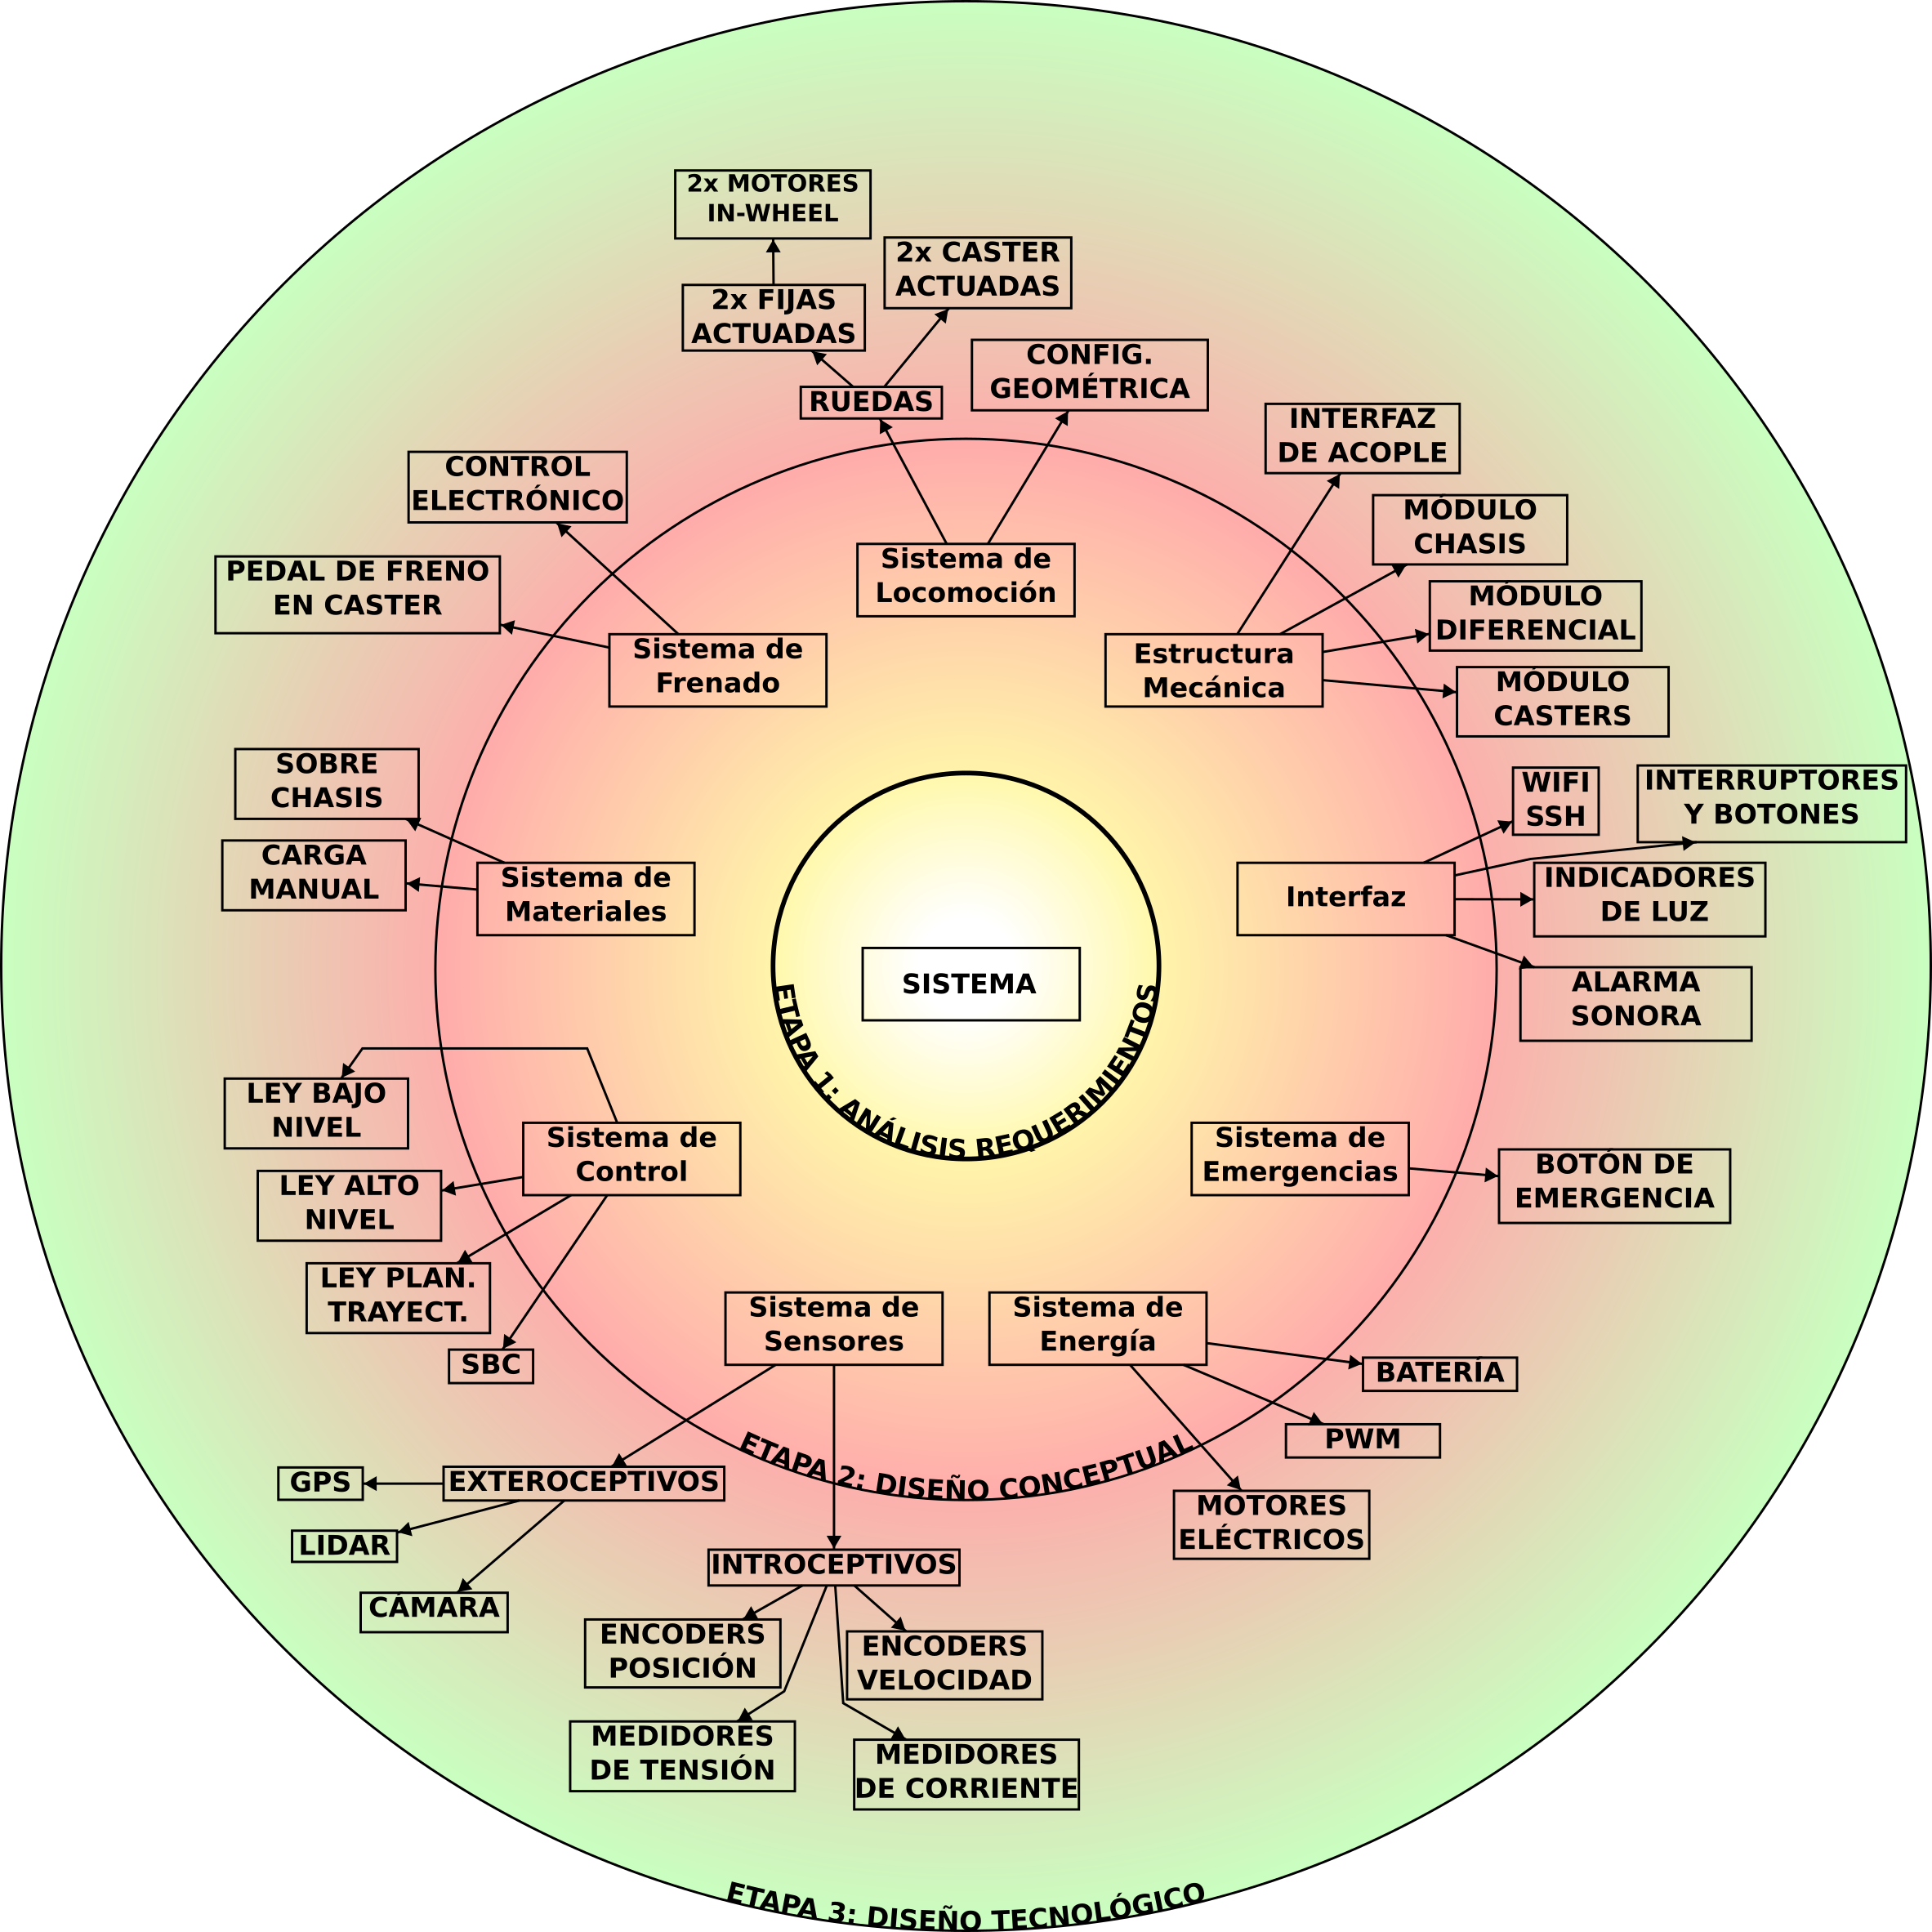
\includegraphics[height=1\textwidth]{figs/onion3.png}
				\end{center}
			\end{column}
			
		\end{columns}
	}

	\designlayer{Diseño Tecnológico}{dl:tecnológico}
	
	\subsubsection{Sistema de Locomoción/Ruedas}
	\frame[t]{\frametitle{\insertsubsubsectionhead}
		{\small \par
		Para iniciar con el proceso de dimensionamiento, se toman algunas estimaciones.
		
		De acuerdo con los requerimientos del entorno, las irregulirades del suelo puede ser de hasta 1.5cm. Una primer aproximación para el radio de las ruedas, es que la pendiente que debe superar ante un escalón de esta magnitud, no supere un ángulo de $45^\circ$.
		\par}
		
		\begin{center}
			%			\pendpres{Mejorar Imágenes}
			%\centering
			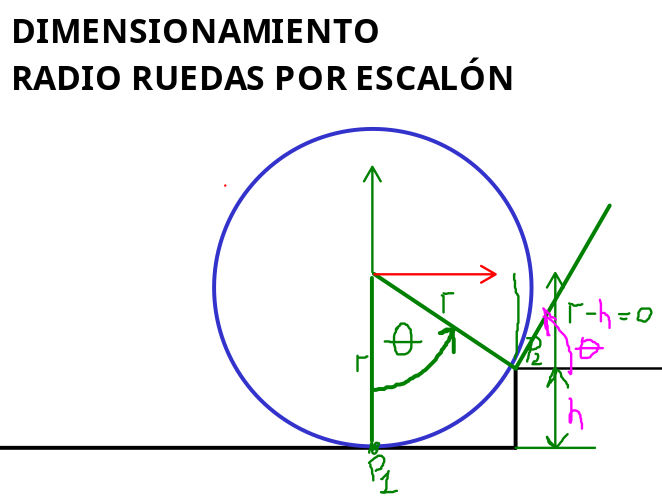
\includegraphics[height=0.4\textheight]{figs/rueda_radioescalon.png}
			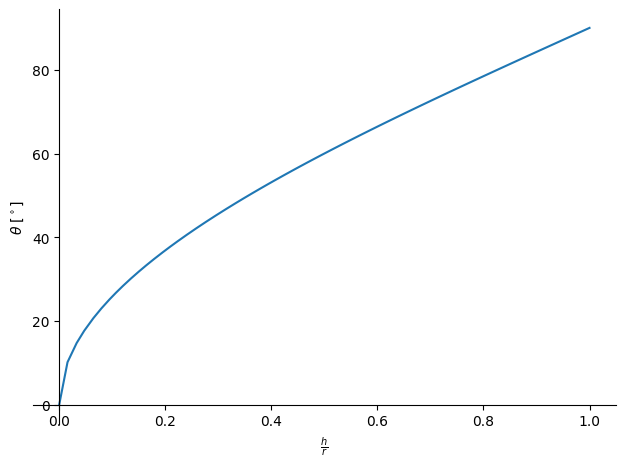
\includegraphics[height=0.4\textheight]{figs/rueda_radioescalongraph.png}
		\end{center}
		
		{\small Para $h=1.5cm$ y $\theta=45^\circ$, se tiene que $\diameter \geq 10cm$}
	}
	
	\subsubsection{Sistema de Locomoción/Disposición}
	\frame[c]{
		\frametitle{\insertsubsubsectionhead}
%		{\small \smaller En las siguientes imágenes de posibles combinaciones de ubicación de las ruedas, el cuadro verde representa el tamaño de la carga (según requerimientos)}
		\begin{columns}[b]
			\begin{column}{.45\textwidth}
				\begin{figure}[H]
					\centering
					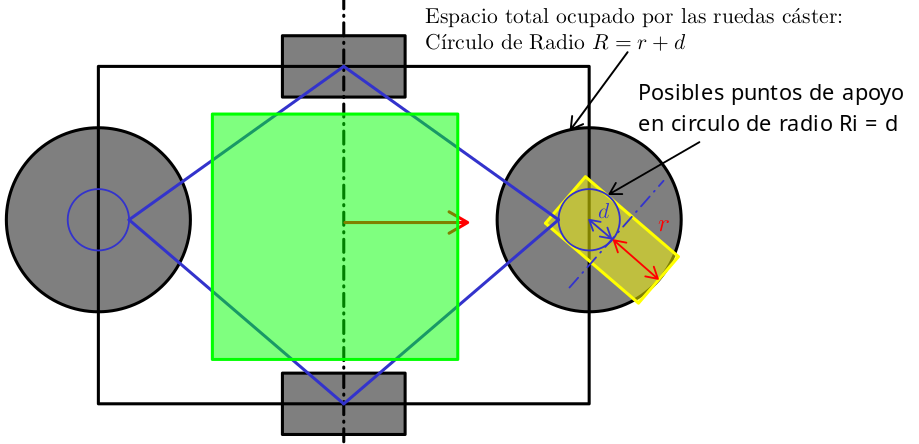
\includegraphics[width=1\textwidth]{figs/loco_dispo_central.png}
					\caption{\small Central}
					%	\label{fig:contextodelsistema}
				\end{figure}
			\end{column}
			\begin{column}{.275\textwidth}
				\begin{figure}[H]
					\centering
					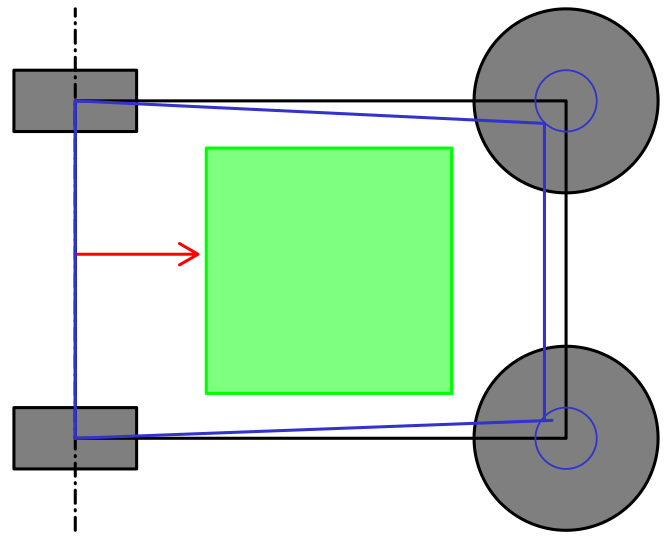
\includegraphics[width=1\textwidth]{figs/loco_dispo_trasera.png}
					\caption{\small Trasera}
					%	\label{fig:contextodelsistema}
				\end{figure}
			\end{column}
			\begin{column}{.275\textwidth}
			\begin{figure}[H]
				\centering
				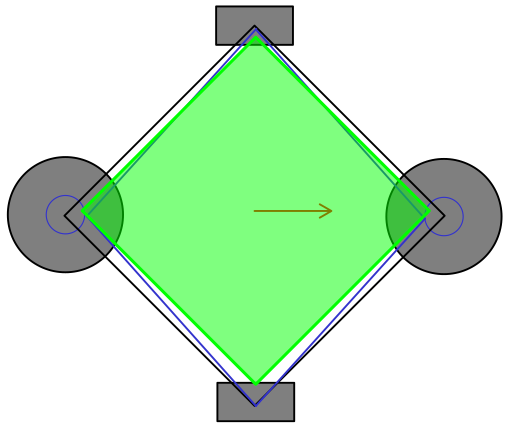
\includegraphics[width=1\textwidth]{figs/loco_dispo_diamante.png}
				\caption{\small Diamante}
				%	\label{fig:contextodelsistema}
			\end{figure}
			\end{column}
		\end{columns}
		\begin{columns}[b]
			\begin{column}{.25\textwidth}
				\begin{figure}[H]
					\centering
					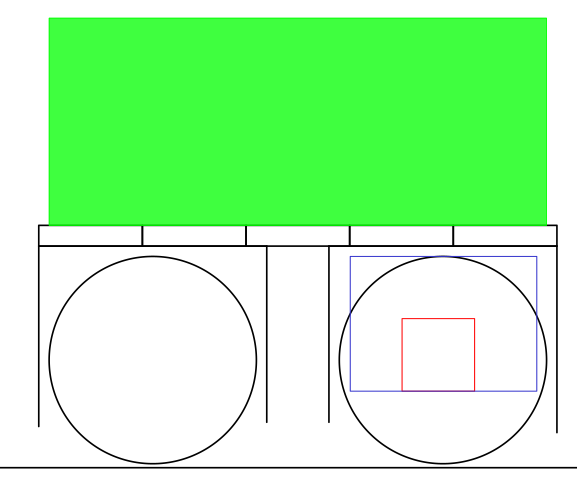
\includegraphics[width=1\textwidth]{figs/loco_dispo_alta.png}
					\caption{\small Alta}
					%	\label{fig:contextodelsistema}
				\end{figure}
			\end{column}
			\begin{column}{.45\textwidth}
				\begin{figure}[H]
					\centering
					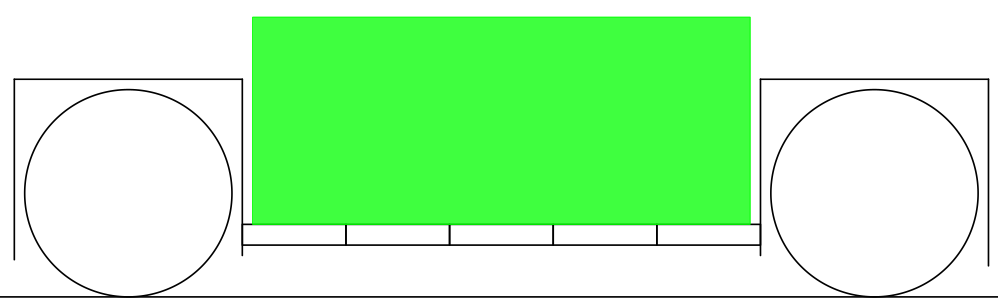
\includegraphics[width=1\textwidth]{figs/loco_dispo_baja.png}
					\caption{\small Baja}
					%	\label{fig:contextodelsistema}
				\end{figure}
			\end{column}
		\end{columns}
	}
	
	\frame[t]{
		\frametitle{\insertsubsubsectionhead}
		La disposición con rueda motriz central no puede subir pendientes dado que ésta quedaría en el aire sin un sistema de suspensión.	\\
		
		\begin{center}{
%		\centering
		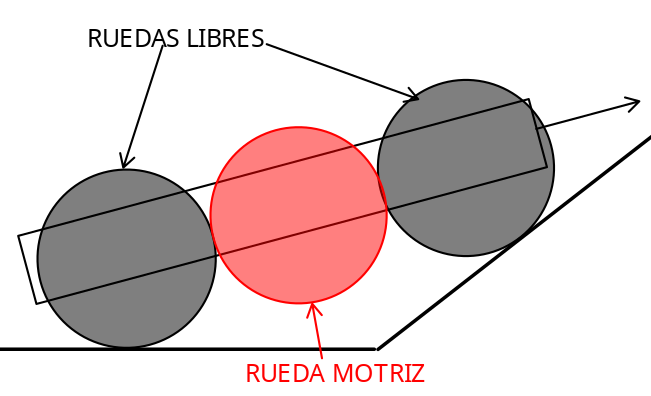
\includegraphics[width=0.5\textwidth]{figs/loco_dispo_centroaire.png}
%		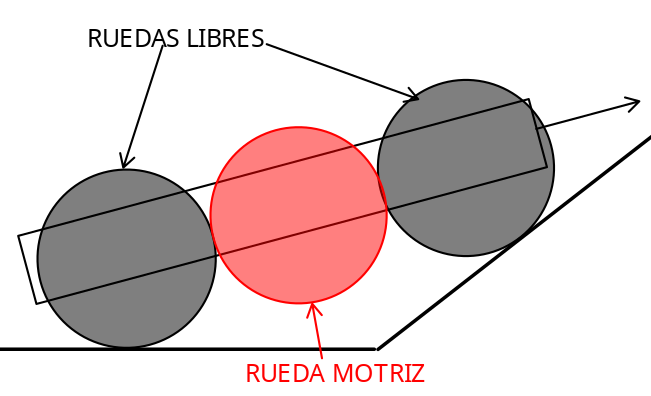
\includegraphics[width=0.45\textwidth]{figs/loco_dispo_centroaire.png}
		}\end{center}
%		\cent
		Se analizan posibles soluciones para estos casos. Se analizan opciones como ruedas neumáticas, de caucho sin aire deformables, sistemas de suspensión con resortes y amortiguadores o rígido utilizando alternativa de configuración trasera.
	}
	
	\frame[t]{ \frametitle{\insertsubsubsectionhead}
		\framesubtitle{Revisitando Etapas Anteriores p/ubicar Sistema de Suspensión}
		\begin{columns}[c]
			\begin{column}{0.5\textwidth}
				Como la solución para esta situación no puede ser descripta por el componente \textbf{Rueda} (salvo si se seleccionaran ruedas neumáticas o deformables), se vuelve hacia atrás en las etapas de diseño para ubicar este componente y evaluar las alternativas.
			\end{column}
			\begin{column}{0.5\textwidth}
				\begin{center}
					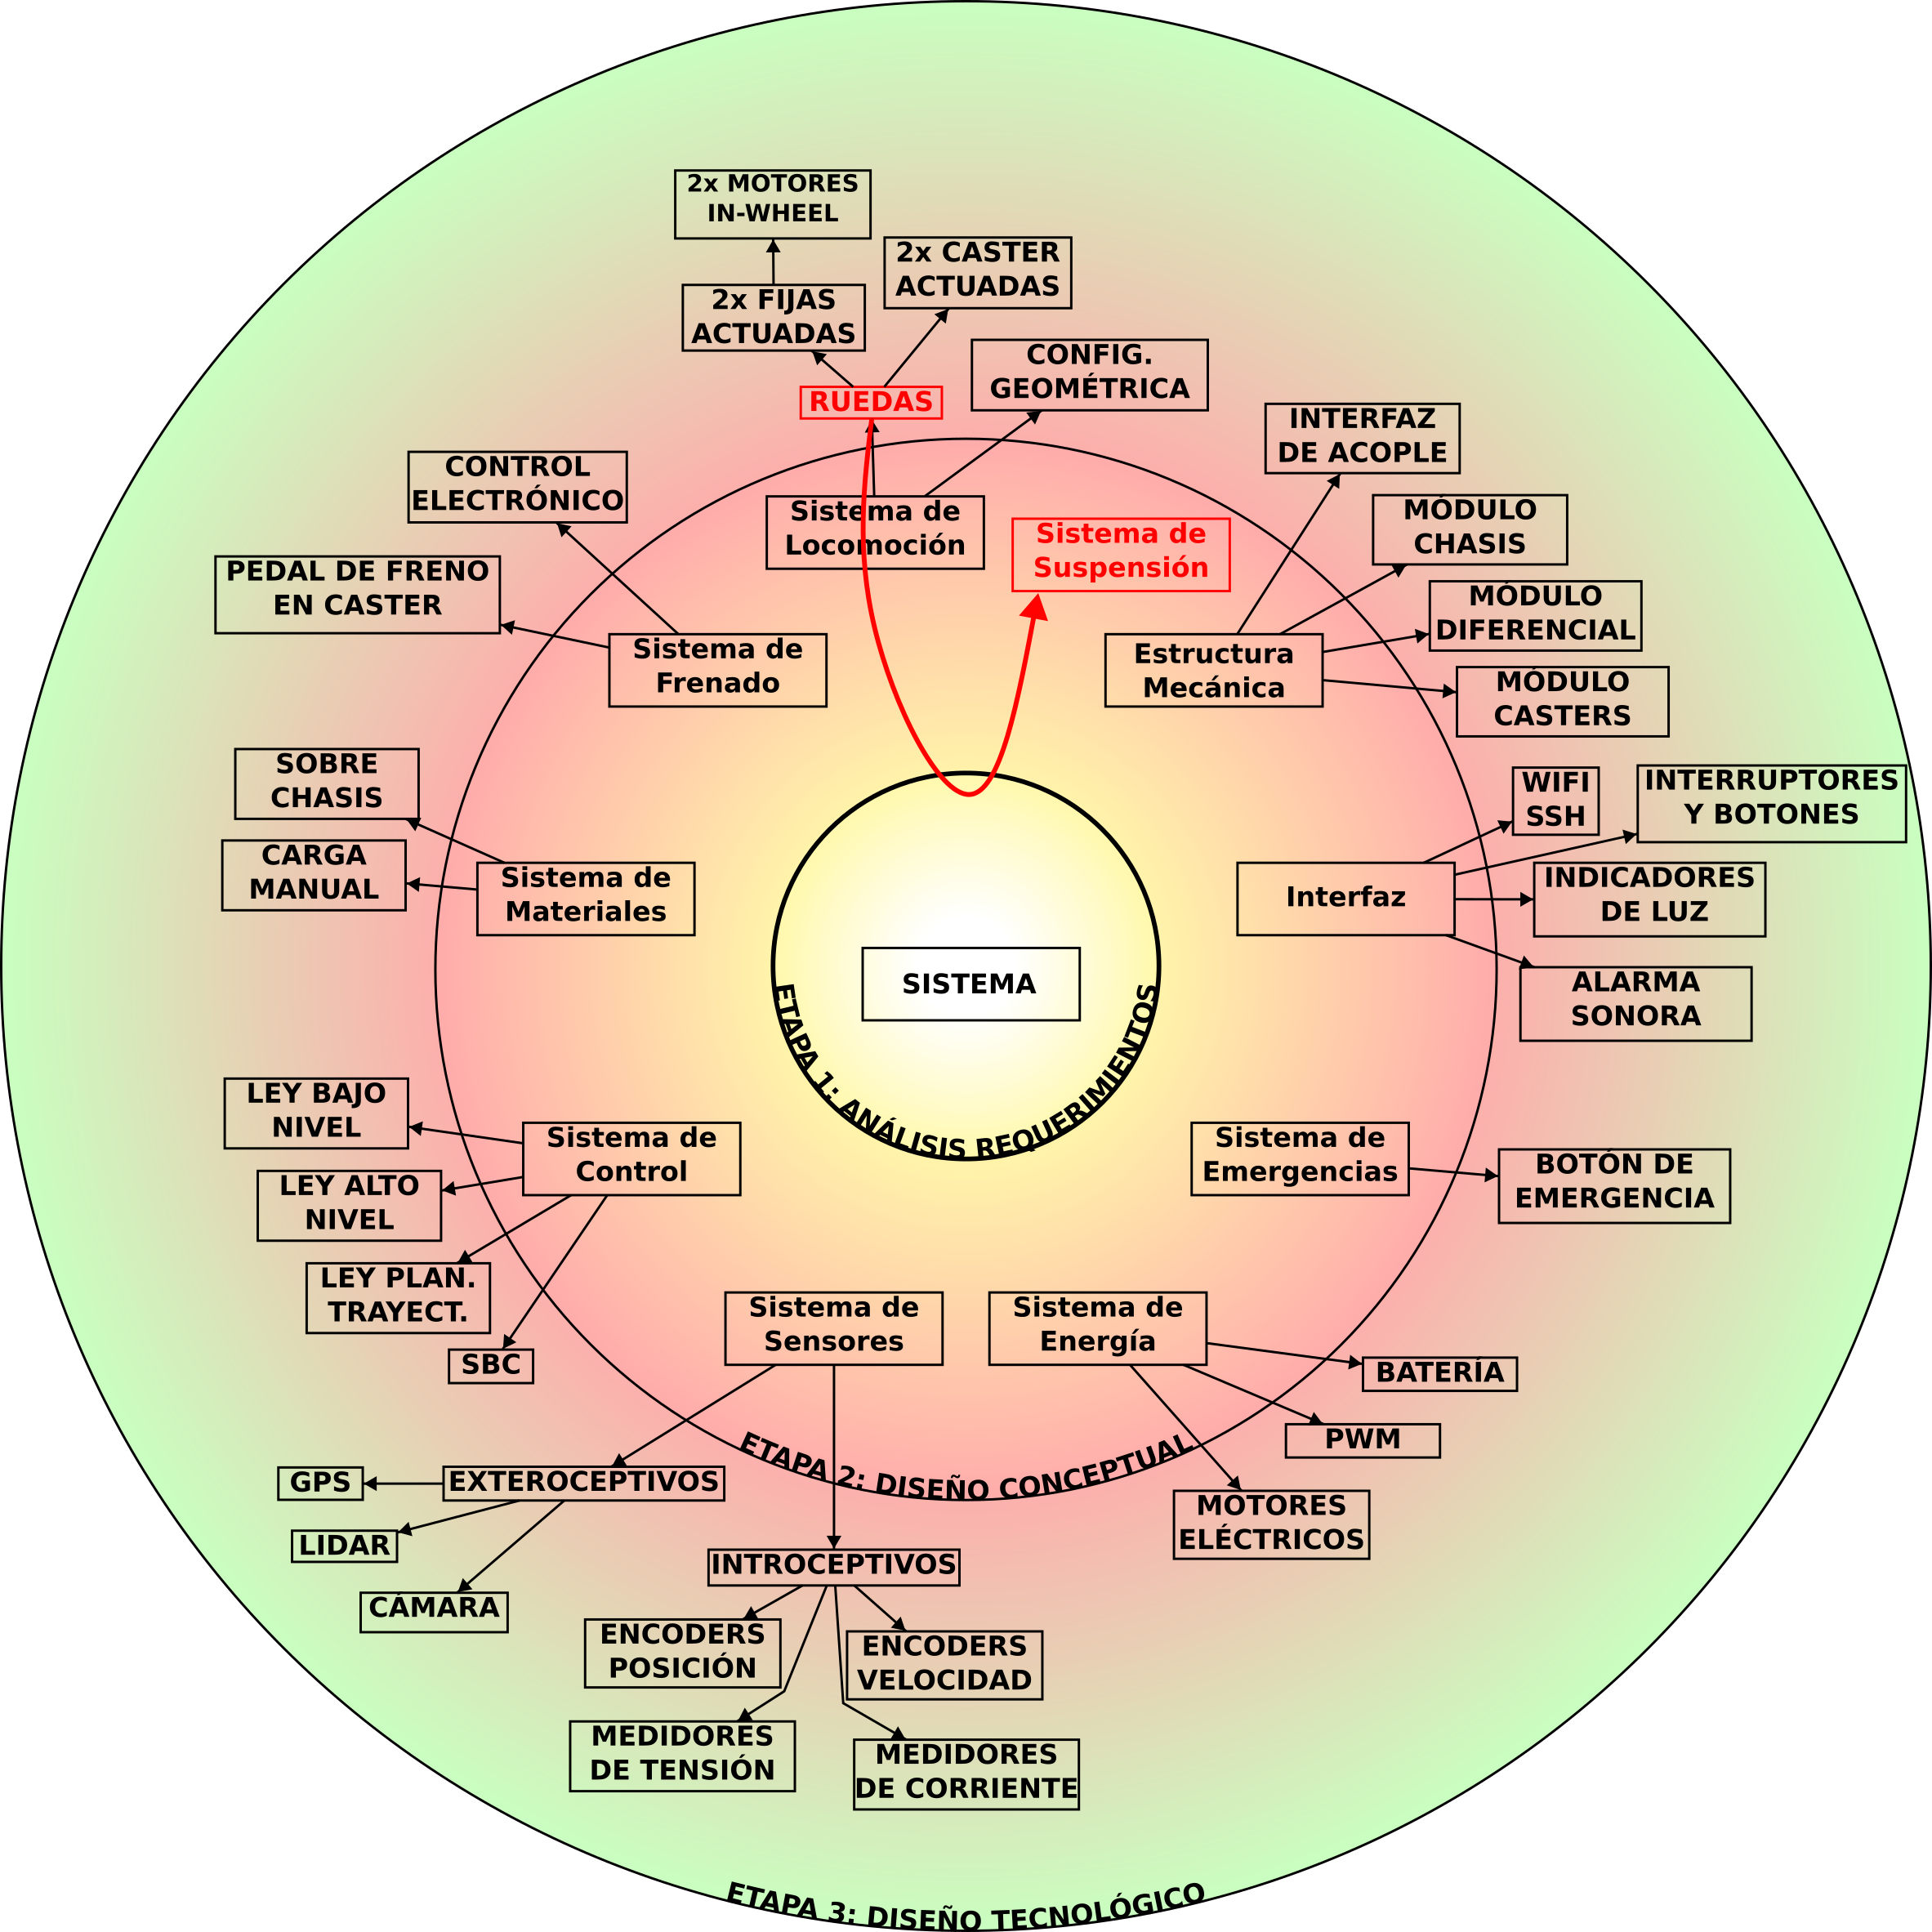
\includegraphics[width=1\textwidth]{figs/onion3_susp.png}
				\end{center}
			\end{column}
			
		\end{columns}
	}
	
	\frame[t]{ \frametitle{Sistema de Suspensión}
		\framesubtitle{Descripción de Alternativas}
		{\par
		\begin{enumerate}\smaller
			\item  \textbf{Rígida: } Sin suspensión. Es necesario garantizar la configuración geométrica para superar obstáculos del terreno y se debe prestar especial atención a impactos y vibraciones de las estructuras mecánicas
			\item \textbf{Ruedas Neumáticas: } La amortiguación y la garantía de contacto con el suelo se hace directamente con un neumático inflado con aire. Como en la fábrica hay mucha viruta metálicas y calientes, esta opción no es muy viable.
			\item \textbf{Ruedas de Caucho Deformables: } La amortiguación se hace directamente en un neumático sólido que se puede deformar. Estas ruedas son caras y se pueden dejar para un segundo nivel del prototipo.
			\item \textbf{Suspensión con Resortes y Amortiguadores: } Complejizan mucho el diseño del prototipo inicial, siendo solucionable con un correcto dimensionamiento y configuración de las ruedas, por lo que esta alternativa es descartada.
		\end{enumerate}
		\par}
	}
	
	\frame[t]{
		\frametitle{\insertsubsubsectionhead}
		\framesubtitle{Volviendo a la disposición geométrica de las ruedas..}
		\textbf{Análisis cinemático de vuelco}
		\begin{columns}[t]
			\begin{column}{0.5\textwidth}
				\small \smaller
				Análisis longitudinal
				\hrule
				\begin{center}
					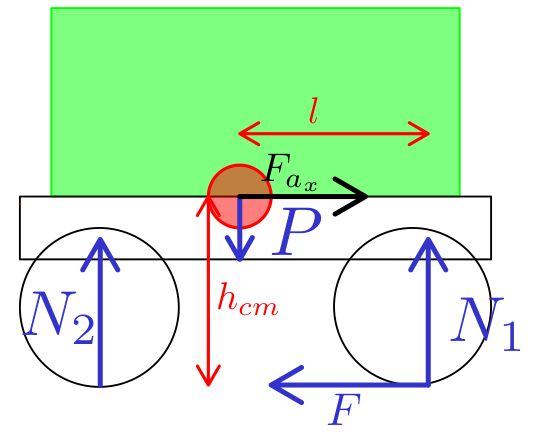
\includegraphics[width=0.5\textwidth]{figs/loco_dispo_vuelco.png}
				\end{center}
				\begin{align*}
					&\text{Fuerza de arrastre: }& F_{a_x} = m_t \cdot a_x  = F\\
					&\text{Momentos respecto a (1): }\\& F_{a_x} \cdot h_{cm} + N_2 \cdot L - P \cdot l = 0 \\
					&\text{Vuelco Inimnente: } N_2 \to 0 & h_{cm} \leq \frac{g\cdot l}{a_x}
				\end{align*}
			\end{column}\begin{column}{0.5\textwidth}
			\small \smaller
				Análogo lateral\par
				\hrule
				\begin{align*}
					&\text{Vuelco Inimnente: } & h_{cm} \leq \frac{g\cdot w}{a_y}
				\end{align*}
				\begin{center}
					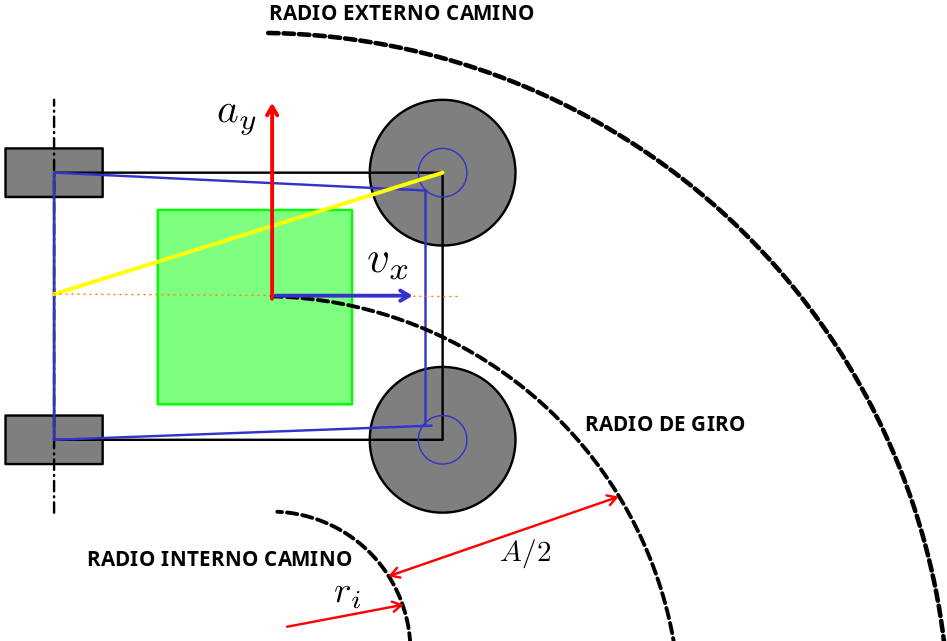
\includegraphics[width=0.7\textwidth]{figs/loco_dispo_vuelcolat.png}
				\end{center}
				\begin{align*}
					&\text{Vuelco Inimnente: } & h_{cm} \leq \frac{g\cdot w \cdot (r_i + A/2)}{v_x^2}
				\end{align*}
			\end{column}
		\end{columns}
	}
	
	\frame[t]{
		\frametitle{\insertsubsubsectionhead}
		\framesubtitle{Análisis cinemático de vuelco}
		
		
		\begin{columns}[t]
			\begin{column}{0.5\textwidth}
				\small
				\smaller
				Utilizando los datos provistos por el cliente:
				\begin{align*}
					v_x &= 2m/s \\
					r_i &= 0.1m \\
					A &= 1m
				\end{align*}
				se obtienen las siguientes relaciones:
				\begin{align*}
					&\text{Longitudinal: } &h_{cm} \leq 4.905 l \\
					&\text{Lateral: } &h_{cm} \leq 0.73575w
				\end{align*}
			\end{column}
			\begin{column}{0.5\textwidth}
				\small
				\begin{center}
					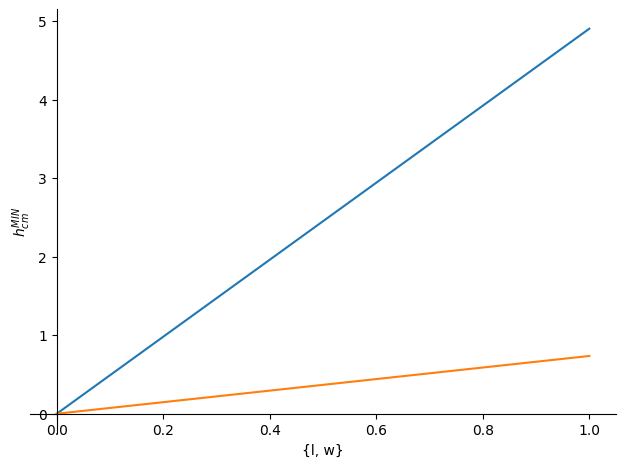
\includegraphics[height=0.4\textheight]{figs/loco_dispo_vuelcograph.png}
				\end{center}
			\end{column}
		\end{columns}
		\hrule
		\bigskip
		\small \smaller
		En base a las restricciones planteadas, dado que la base es esencialmente cuadrada (por la carga cuadrada que debe trasladar), y  para las solicitaciones impuestas para la base móvil, es priotario aumentar el ancho de la base en vez de el largo.
		
		Sin embargo, la aceleración lateral exigida es muy alta, por lo que igualmente se deberá evaluar la posibilidad de disminuir la velocidad de curvas estando cargada.
	}
	
	\frame[t]{
		\frametitle{\insertsubsubsectionhead}
		\textbf{Análisis del despeje mínimo}
	\begin{columns}[t]
		\begin{column}{0.5\textwidth}
			\small \smaller
			\begin{center}{
					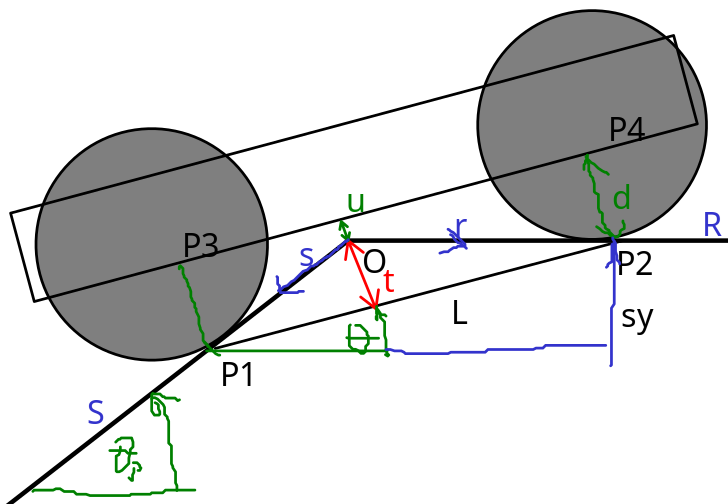
\includegraphics[width=1\textwidth]{figs/loco_dispo_despeje.png}
			}\end{center}
			\begin{equation*}
				d \geq \frac{\left(L \sqrt{1 - \frac{\sin^{2}{\left(\theta_{p} \right)}}{4}} - \frac{L \cos{\left(\theta_{p} \right)}}{2}\right) \sin{\left(\theta_{p} \right)}}{2}	
			\end{equation*}
		\end{column} \begin{column}{0.5\textwidth}
			\small \smaller
			De acuerdo a los requisitos clientes, la base móvil debe superar pendientes de hasta $\theta_p \leq 15^{\circ}$.
			
			Se prevé (modelo predictivo) que la distancia entre ejes no superará $L \leq 1.2m$ para no perder radio de giro.
			
			Con estos datos, el despeje mínimo $d$ es:
			\begin{equation*}
				d \geq 8cm
			\end{equation*} 
		\end{column}
	\end{columns}
	}
		
	
	\subsubsection{Estructura Mecánica/Interfaz de Acople}
	
	\frame[t]{
		\frametitle{\insertsubsubsectionhead}
		\small \smaller
		\textbf{Funciones de la Interfaz de Acople}
		\begin{enumerate}
			\item Permitir vincular distintos módulos de locomoción, estructuras de operación y/o de sensores para cambiar la configuración de uso del Sistema.
			\item Soportar esfuerzos mecánicos que se transmiten a través de los distintos módulos
		\end{enumerate}
		\begin{columns}[t]
			\column{0.5\textwidth}{
				\begin{center}{
						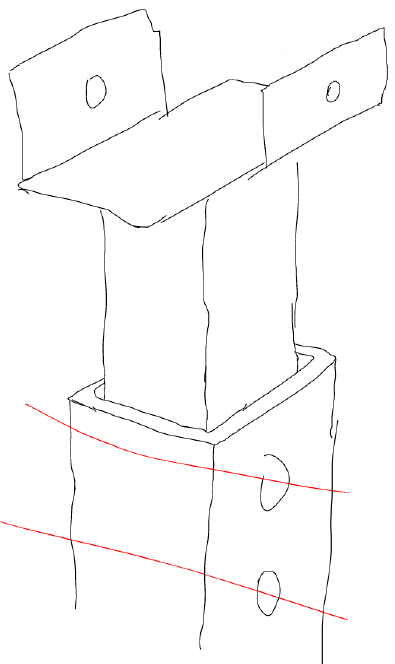
\includegraphics[height=0.6\textheight]{figs/estmec_acople_croquis1.png}
				}\end{center}
			}
			\column{0.5\textwidth}{
				\begin{center}{
						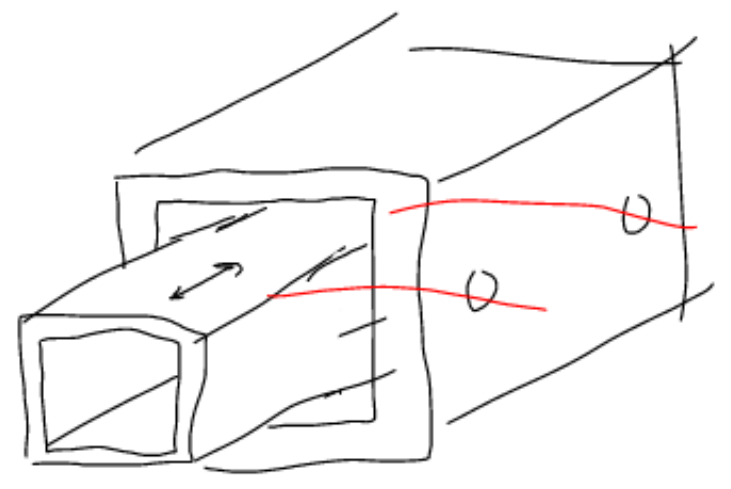
\includegraphics[height=0.25\textheight]{figs/estmec_acople_croquis2.png}
				}\end{center}
				\begin{center}{
						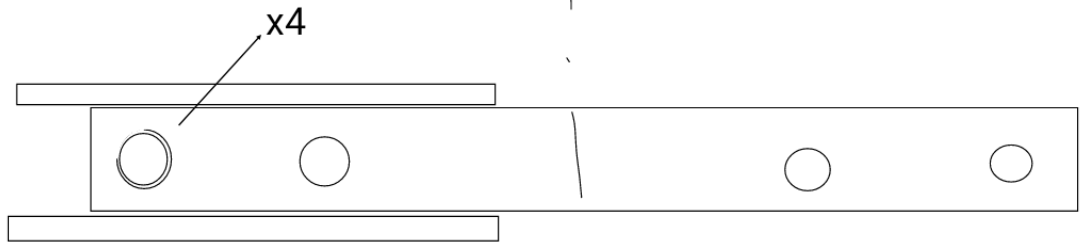
\includegraphics[width=1\textwidth]{figs/estmec_acople_croquis3.png}
				}\end{center}
				}
		\end{columns}
	}
	\frame[t]{
		\frametitle{\insertsubsubsectionhead}
		\small \smaller
		\textbf{División en subcomponentes de la interfaz de acople}
%		\pendpres{Hacer...}
		\begin{enumerate}
			\item Caño hembra
			\item Caño Macho
			\item Tornillos y tuercas
			\item Interfaz externa
		\end{enumerate}
		
		\textbf{Especificación de funcionalidades, requerimientos, métodos de verificación y dimensionamientos}
	}
	
	\designlayer{Diseño Detallado}{dl:detallado}
	\frame[t]{
		\begin{columns}[t]
			\column{0.5\textwidth}{
				\small \smaller
				\textbf{Análisis de funcionalidades y requerimientos de cada componente:}\\
				solicitaciones mecánicas, reconfigurabilidad, etc.
				\begin{center}{
						
						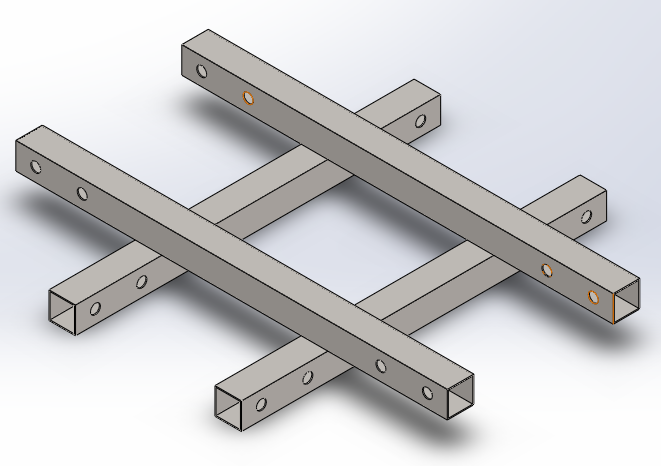
\includegraphics[width=1\textwidth]{figs/disdet_chasis.png}
						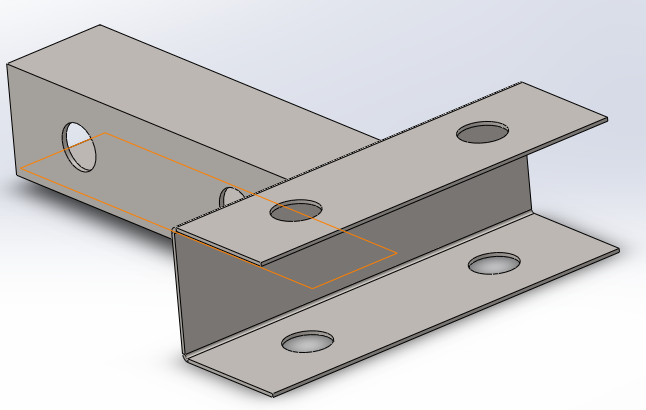
\includegraphics[width=0.45\textwidth]{figs/disdet_acople1.png}
						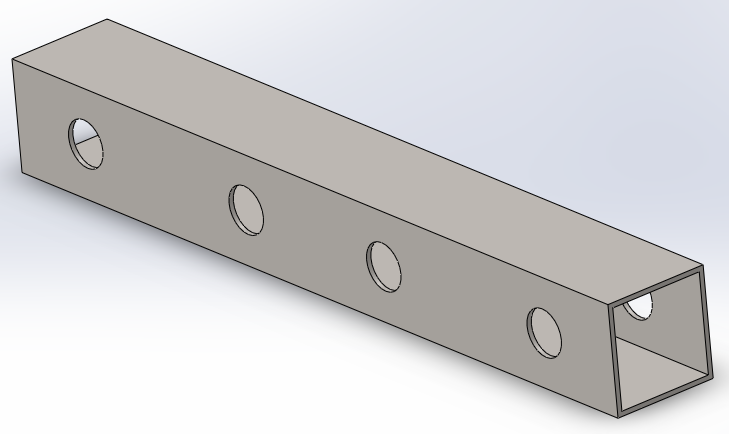
\includegraphics[width=0.5\textwidth]{figs/disdet_acople2.png}
				}\end{center}
			}
			\column{0.5\textwidth}{
				\begin{center}{
						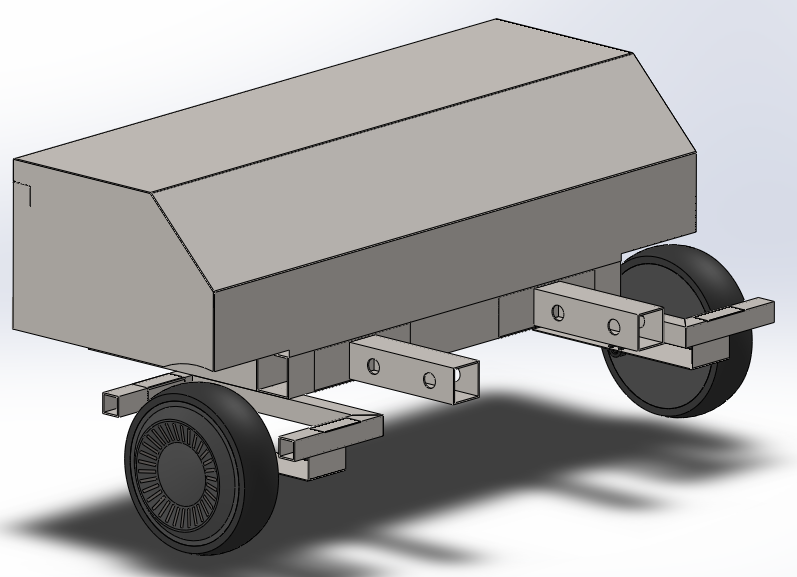
\includegraphics[width=0.85\textwidth]{figs/disdet_difs.png}
				}\end{center}
				\begin{center}{
						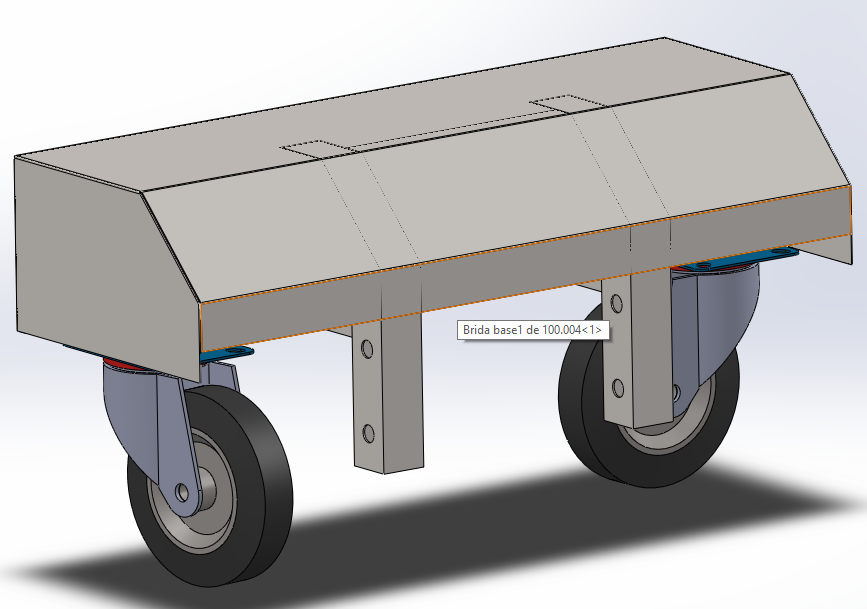
\includegraphics[width=0.85\textwidth]{figs/disdet_casters.png}
				}\end{center}
			}
		\end{columns}
	}
	
	\section{Resultados}
	
	\subsection{Integración, validación y verificación}
	\frame[t]{
	\begin{columns}[t]
		\column{0.5\textwidth}{
			\small 
%			\textbf{Integración: } \\
			\smaller Los componentes diseñados deben integrarse entre sí, y se debe verificar y validar todos los requisitos heredados de las etapas anteriores, por ejemplo:
			\begin{enumerate}
				\item Despeje del suelo
				\item Aceleraciones máximas al vuelco
				\item Resistencia mecánica de las interfaces de acople y de los módulos
				\item Capacidad de superar irregularidades del terreno
				\item Autonomía
				\item Reconfigurabilidad
				\item etc.
			\end{enumerate}
		}
		\column{0.5\textwidth}{
			\begin{center}{
					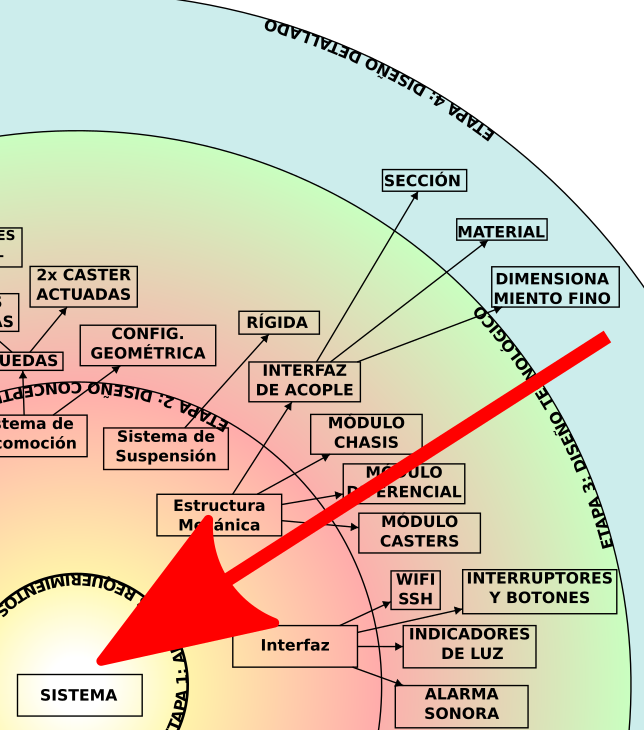
\includegraphics[width=1\textwidth]{figs/onion4.png}
			}\end{center}
		}
	\end{columns}
	}
	
	\frame[t]{
		\begin{columns}[t]
			\column{0.4\textwidth}{
				\begin{center}{
						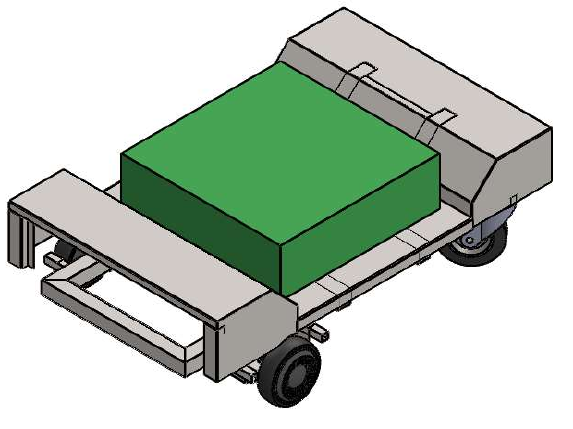
\includegraphics[height=0.4\textheight]{figs/res_iso1.png}
						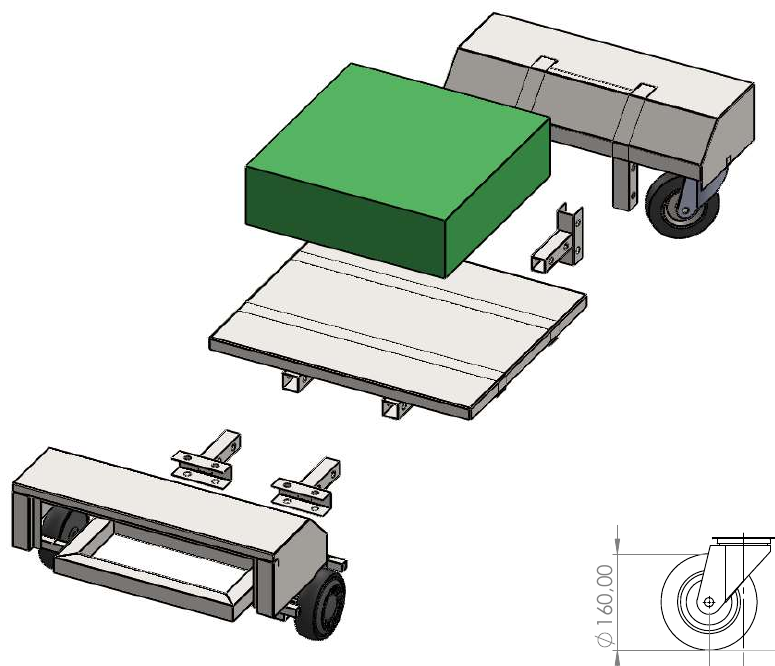
\includegraphics[height=0.4\textheight]{figs/res_desplegado.png}
				}\end{center}
			}
			\column{0.6\textwidth}{
				\begin{center}{
						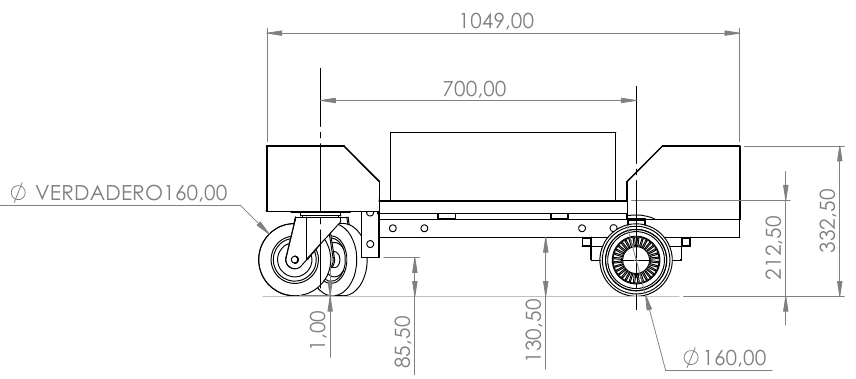
\includegraphics[width=1\textwidth]{figs/res_lateral.png}
				}\end{center}
				\begin{center}{
						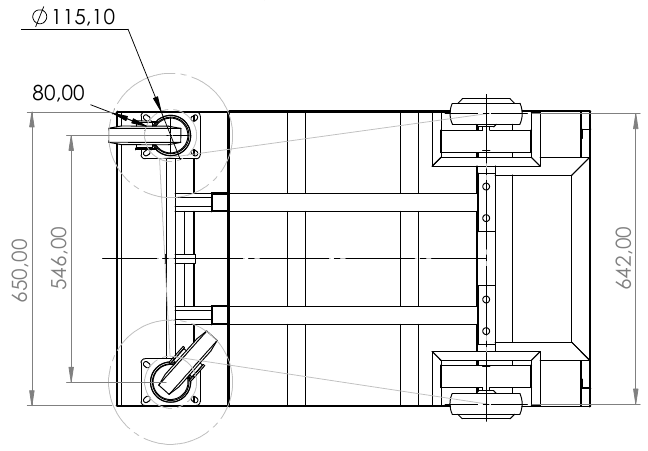
\includegraphics[width=0.85\textwidth]{figs/res_inferior.png}
				}\end{center}
			}
		\end{columns}
	}
	
	\subsection{Comparación con Diseño Previo}
	\frame[t]{
		\begin{columns}[t]
			\column{0.5\textwidth}{
				\small \smaller 
				El diseño original se hizo sin utilizar metodologías de diseño sofisticadas como las desarrolladas en esta presentación y eso implica que el diseño puede resultar con muchas falencias que son más difíciles de resolver al no disponer de trazabilidad de diseño.
				
				Si bien no el nuevo diseño no está terminado, ya se puede evidenciar algunas mejoras respecto al diseño anterior:
				\begin{enumerate}
					\item Tiene mejor estabilidad sin ocupar mucho más espacio físico
					\item Tiene mucha más perspectiva de reconfiguración y de integración (por ejemplo, espacio para la electrónica)
					\item El proceso de diseño detallado se hace con mayor cantidad de restricciones y permite mayor seguridad durante la toma de decisiones
				\end{enumerate}
			}
			\column{0.5\textwidth}{
				\begin{center}{
						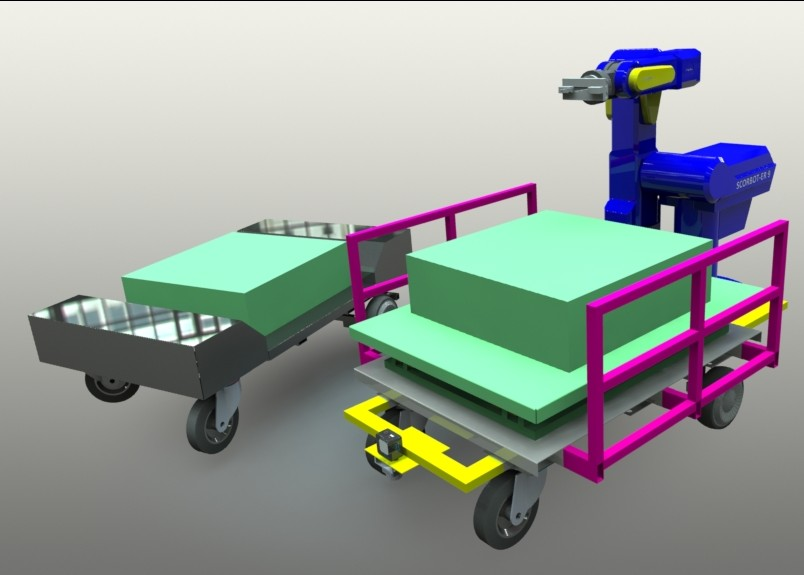
\includegraphics[width=1\textwidth]{figs/render.png}
				}\end{center}
			}
		\end{columns}
	}
	
	\section{Conclusiones}
	
	
%	\appendix
%%	\appendixtocon
%	\section{Apéndice}
%	\subsection{asd}
	
	%% LIST OF TODOs
%	\frame[t]{
%		\listoftodos
%	}

%	\section{Referencias}
	\frame[t]{ \frametitle{Referencias}
		\small \smaller
		\nocite{vitolo_mobile_2022}
		\nocite{couturier_tracking_2014}
		\nocite{cw_de_silva_design_2013}
		\nocite{moulianitis_new_2018}
		\nocite{fulop_introduction_nodate}
		\bibliographystyle{plain}
		\bibliography{2403-biblio.bib}
	}
	
\end{document}